\documentclass[a5paper,oneside]{amsart}
\usepackage[scale={.9,.8}]{geometry}
\usepackage{mathrsfs}
\usepackage{amsthm}
\usepackage{amsmath}
\usepackage{amsfonts}
\usepackage{graphicx}
\usepackage{dsfont}
\usepackage{listings}
\usepackage[spanish,mexico]{babel}
\usepackage[latin1]{inputenc}
\theoremstyle{plain}
\newtheorem{theorem}{Theorem}
\newtheorem{lemma}{Lemma}
\newtheorem{corollary}{Corollary}
\newtheorem{proposition}{Proposition}
\newtheorem{conjecture}{Conjecture}
\theoremstyle{definition}
\newtheorem{problema}{Problema}
%\newtheorem{problema}{Ejercicio}
\newtheorem*{definition}{Definition}
\newtheorem*{remark}{Remark}
\usepackage{enumitem}
\usepackage{listings}
\lstset{
language=R,
basicstyle=%\scriptsize
\ttfamily,
commentstyle=\ttfamily\color{gray},
numbers=none,
numberstyle=\ttfamily\color{gray}\footnotesize,
stepnumber=1,
numbersep=5pt,
backgroundcolor=\color{white},
showspaces=false,
showstringspaces=false,
showtabs=false,
frame=none,
tabsize=4,
captionpos=b,
breaklines=true,
breakatwhitespace=false,
title=\lstname,
escapeinside={},
keywordstyle={},
morekeywords={}
}
\title[Problemas de Procesos I]{Problemas de Procesos Estoc\'asticos I\\ Semestre 2013-II\\ Posgrado en Ciencias Matem\'aticas\\ Universidad Nacional Aut\'onoma de M\'exico}
\author{Ger\'onimo Uribe Bravo}
%\address{}
\usepackage[colorlinks,citecolor=blue,urlcolor=blue]{hyperref}
%\setlength{\textwidth}{17.2cm} % was 18.2
%\setlength{\textheight}{23cm} % was 23
%\setlength{\torgin}{-1cm} % was 0
%\setlength{\oddsidemargin}{-0.6cm}
%\setlength{\evensidemargin}{-0.6cm}

%\setlength{\textwidth}{18.9cm} % was 18.2
%\setlength{\textheight}{26.73cm} % was 23
%\setlength{\topmargin}{1cm} % was 0
%\setlength{\oddsidemargin}{0cm} %
%\setlength{\evensidemargin}{.8cm}
%% Arreglar pues ahora utilizas papel A4.

%Operadores

\DeclareMathOperator{\ivp}{IVP} %
\DeclareMathOperator{\sgn}{sgn} %
\DeclareMathOperator{\md}{mod}
\DeclareMathOperator{\ima}{Im}%
\DeclareMathOperator{\id}{Id} %
\DeclareMathOperator{\homo}{Hom} %
\DeclareMathOperator{\inter}{Int}
\DeclareMathOperator*{\Lim}{lim}
\DeclareMathOperator*{\Limsup}{lim\ sup}
\DeclareMathOperator*{\Liminf}{lim\ inf}
\DeclareMathOperator*{\Min}{m\text{\ii}n}
\DeclareMathOperator{\Aff}{Aff}
\DeclareMathOperator{\Affb}{\overline{\Aff}}
\DeclareMathOperator{\sdfd}{dfd}
\DeclareMathOperator{\scdfd}{dfd}
\DeclareMathOperator{\Beta}{B}
\DeclareMathOperator{\pd}{PD}
\DeclareMathOperator{\supp}{supp}
\DeclareMathOperator{\diam}{diam}
\newcommand{\ind}{\operatornamewithlimits{\perp}}
\DeclareMathOperator{\av}{Abs}
\DeclareMathOperator{\cb}{CB}
\DeclareMathOperator{\cbi}{CBI}
\DeclareMathOperator{\gwi}{GWI}
\DeclareMathOperator{\gw}{GW}
\newcommand{\rtree}{$\re$\nbd tree}
\newcommand{\leb}{\text{Leb}}
%Notaci�n



%Delimitadores
\newcommand{\ceil}[1]{\ensuremath{\lceil #1 \rceil}}
%\renewcommand{\floor}[1]{\ensuremath{\lfloor #1 \rfloor}}

%Formato
\newcommand{\defin}[1]{{\bf #1}}
\newcommand{\mc}[1]{\ensuremath{\mathscr{#1}}}
\newcommand{\bb}[1]{\mathbb{#1}}


%Notation

\newcommand{\card}[1]{\ensuremath{\left| #1 \right|}}
\newcommand{\lccb}{LCCB}
\newcommand{\pss}{S}
\newcommand{\compact}{K}
\newcommand{\psm}{\rho}
\newcommand{\ps}{\paren{\pss,\psm}}
\newcommand{\pse}{x}
\newcommand{\psep}{y}
\newcommand{\psepp}{z}
\newcommand{\saps}{\B_{\pss}}
\newcommand{\bre}{\B_{\re}}
\newcommand{\sko}{D}
\newcommand{\trees}{T}
\newcommand{\C}{C}
\newcommand{\refm}{\mu}
\newcommand{\den}{p}
\newcommand{\psd}[1]{\mc{P}_{#1}}
\newcommand{\s}{\ensuremath{\sigma}}
\newcommand{\bden}{M}
\newcommand{\hh}[1]{{\bf H#1}}
\newcommand{\ball}[2]{\imf{B_{#1}}{#2}}
\newcommand{\mmc}[1]{\imf{\tilde\omega}{#1}}
\newcommand{\rg}[1]{\ensuremath{\imf{\mathbb{G}}{#1}}}




\newcommand{\dfd}{\ensuremath{\stackrel{\sdfd}{=}}}
\newcommand{\deq}{\ensuremath{\stackrel{d}{=}}}

\newcommand{\ley}[2]{\ensuremath{\imf{\mc{L}^{#2}}{#1}}}
\newcommand{\leyc}[3]{\ensuremath{\imf{\mc{L}^{#3}}{#1\left|#2\right.}}}
\newcommand{\cond}[2]{\left.\vphantom{#2}#1\ \right| #2}

\newcommand{\e}{\ensuremath{\mathbf{e}}}
\newcommand{\esf}{\ensuremath{\mc{S}^{\downarrow}}}
%\newcommand{\ps}[1]{\mathscr{P}\paren{#1}}
\newcommand{\fun}[3]{\ensuremath{#1:#2\to #3}}
\newcommand{\fund}[3]{\ensuremath{#1:#2\mapsto #3}}
\newcommand{\set}[1]{\ensuremath{\left\{ #1\right\} }}
\newcommand{\sets}[1]{\ensuremath{{\mathbf #1}}}
\newcommand{\paren}[1]{\ensuremath{\left( #1\right) }}
\newcommand{\bra}[1]{\ensuremath{\left[ #1\right] }}
\newcommand{\seq}[1]{\ensuremath{ #1 _1,\ldots ,#1 _n }}
\newcommand{\sm}[3]{\left[ #1\right]_{#2}^{#3}}
\newcommand{\cde}{\Rightarrow}
\newcommand{\cdfd}{\ensuremath{\stackrel{\scdfd}{\cde}}}
\newcommand{\convo}[2]{\ensuremath{#2^{\!* #1}}}

\newcommand{\tl}[1]{\ensuremath{\hat{#1}}}

\newcommand{\matt}[3]{#1_{#2\, #3}}
\newcommand{\sip}{\bb{P}}
\newcommand{\jump}[2]{\ensuremath{\Delta #1_{#2}}}
\newcommand{\cadlag}{c\`adl\`ag}
\newcommand{\se}{\ensuremath{\bb{E}}}
\newcommand{\ssa}{\ensuremath{\mathscr{F}}}
\newcommand{\si}{{\ensuremath{\bf{1}}}}
\newcommand{\sbr}{\ensuremath{\mc{B}_{\re}}}
%\newcommand{\siind}{\ensuremath{\perp}}
\newcommand{\sigam}{\ensuremath{\Gamma}}
\newcommand{\smc}{\ensuremath{m}}
\newcommand{\sfleche}{S^{\downarrow}_f}

\newcommand{\gafun}[1]{\sigam \paren{#1}}
\newcommand{\poi}[1]{\ensuremath{\mc{P}\!_{#1}}}
\newcommand{\ber}[1]{\ensuremath{\mc{B}\!_{#1}}}
\newcommand{\fcpoi}[1]{\ensuremath{\hat{\mc{P}}\!_{#1}}}
%\newcommand{\ind}{\siind}
\newcommand{\condind}[3]{\ensuremath{#1\ind_{#3}#2}}
\newcommand{\sig}[1]{$\sigma$-\nobreakdash #1}
\newcommand{\sa}{\ensuremath{\sigma}\nbd field}
\newcommand{\realtree}{\ensuremath{\re}\nbd tree}
\newcommand{\eps}{\ensuremath{ \varepsilon}}
\newcommand{\na}{\ensuremath{\mathbb{N}}}
\newcommand{\en}{\ensuremath{\mathbb{Z}_+}}
\newcommand{\eti}{\ensuremath{\mc{U}}}
\newcommand{\etic}{\ensuremath{\mathbb{U}}}
\newcommand{\z}{\ensuremath{\mathbb{Z}}}
\newcommand{\re}{\ensuremath{\mathbb{R}}}
\newcommand{\ra}{\ensuremath{\mathbb{Q}}}
\newcommand{\com}{\ensuremath{\mathbb{C}}}
\newcommand{\con}[1]{\ensuremath{\overline{#1}}}
\newcommand{\proba}[1]{\ensuremath{\sip\! \left( #1 \right)}}
\newcommand{\probas}[2]{\ensuremath{#1\! \left( #2 \right)}}
\newcommand{\probac}[2]{\ensuremath{\sip\! \left( #1 \, | #2 \right)}}
\newcommand{\esp}[1]{\ensuremath{\se\! \left( #1 \right)}}
%\newcommand{\espc}[2]{\ensuremath{\se\! \left( #1 | #2 \right)}}
\newcommand{\espc}[2]{\ensuremath{\imf{\se}{\cond{#1}{#2}}}}
\newcommand{\var}[1]{\ensuremath{\text{Var}\! \left( #1 \right)}}
\newcommand{\cov}[1]{\ensuremath{Cov\! \left( #1 \right)}}
\newcommand{\abs}[1]{\hspace{.25mm}\left|#1\right|\hspace{.25mm}}
\newcommand{\ila}[2]{\ensuremath{\int #1\, d#2}}
\newcommand{\ilas}[3]{\ensuremath{\int_{#1} #2\, d#3}}
\newcommand{\il}[3]{\ensuremath{\int #1\, \imf{#2}{d#3}}}
\newcommand{\is}[4]{\ensuremath{\int_{#1} #2\, \imf{#3}{d#4}}}
\newcommand{\lp}[2]{\ensuremath{\mc{L}_#1\!\paren{#2} }}
\newcommand{\lpc}[4]{\ensuremath{\mc{L}_#1\!\paren{ #2 , #3 , #4 }}}
\newcommand{\ip}[1]{\ensuremath{\int #1\, d\sip }}
\newcommand{\ips}[2]{\ensuremath{\int_{#1} #2\, d\sip}}
\newcommand{\F}{\ssa}
\newcommand{\uF}{\ssa^u}
\newcommand{\G}{\ensuremath{\mc{G}}}
\newcommand{\h}{\ensuremath{\mc{H}}}
\newcommand{\B}{\ensuremath{\mc{B}}}
\newcommand{\f}[1]{\ssa_{#1}}
\newcommand{\fx}[2]{\ssa_{#1}^{#2}}
\newcommand{\indi}[1]{\si_{#1}}
\newcommand{\imi}[2]{#2^{-1}\!\paren{#1}}
\newcommand{\ooo}{\ensuremath{ \omega  } }
\newcommand{\oo}{\ensuremath{ \Omega  } }
\newcommand{\p}{\ensuremath{ \sip  } }
\newcommand{\q}{\ensuremath{ \bb{Q}  } }
\newcommand{\ofp}{\ensuremath{ \paren{ \Omega ,\F ,\p } } }
\newcommand{\med}[2]{\ensuremath{\paren{#1}{#2}}-medible}
\newcommand{\vat}{\ensuremath{\fun{X}{\oo}{\re}}\ }
\newcommand{\pix}[1]{\ensuremath{\sip}_{\! #1}}
\newcommand{\px}[2]{\ensuremath{\sip_{\! #1}\!\paren{#2}}}
\newcommand{\pxc}[3]{\ensuremath{\sip_{\! #1}\!\left( #2 | #3 \right)}  }
\newcommand{\br}{\sbr}
\newcommand{\sag}[1]{\sigma\!\paren{#1}}
\newcommand{\cs}[1]{\ensuremath{#1}-p.s.}
\newcommand{\ore}{ \ensuremath{\overline{\re}}}
\newcommand{\fungen}[1]{\ensuremath{\varphi_{#1}}}%Comando para la notaciÛn de funciÛn generadora.
\newcommand{\cbin}[2]{\ensuremath{\paren{\begin{array}{c}#1\\#2\end{array}}}}
\newcommand{\fa}[2]{\ensuremath{{#1}^{\paren{#2}}}}
\newcommand{\dnor}[2]{\ensuremath{N(#1,#2)}}
\newcommand{\mb}{movimiento browniano}
\newcommand{\moc}[3]{\smc^{#3}(#1,#2)}
\newcommand{\clo}[1]{\ensuremath{\overline{#1}}}
\newcommand{\inte}[1]{\ensuremath{\inter #1}}
\newcommand{\fro}[1]{\ensuremath{\partial\paren{ #1}}}
\newcommand{\cd}[2]{\ensuremath{#1\stackrel{\mc{D}}{\to}#2}}
\newcommand{\pr}[3]{\ensuremath{#1_{#2}\!\paren{#3}}}
\newcommand{\oi}[1]{\ensuremath{\mc{O}\paren{#1}}}
\newcommand{\mw}{\ensuremath{\mathbb{P}}}
\newcommand{\me}{\ensuremath{\pi}}


\newcommand{\nbd}{\nobreakdash -}
\newcommand{\ii}{\'{\i}}
\newcommand{\n}{\~n}
\newcommand{\imf}[2]{\ensuremath{#1\!\paren{#2}}}
\newcommand{\floor}[1]{\ensuremath{\lfloor #1\rfloor}}
\newcommand{\proint}[2]{\ensuremath{\langle #1,#2\rangle}}
\newcommand{\vp}{\ensuremath{\varphi}}
\newcommand{\noru}[1]{\ensuremath{\|#1\|}}
\newcommand{\gen}[1]{\ensuremath{|#1 |}}
\newcommand{\vc}[1]{\ensuremath{\langle #1\rangle}}
\newcommand{\pc}[2]{\ensuremath{\langle#1,#2\rangle}}
\newcommand{\vcd}[1]{\ensuremath{\left[#1\right]}}

\newcommand{\sml}{\ensuremath{\nu}}
\newcommand{\ml}[1]{\ensuremath{\imf{\sml}{#1}}}
\newcommand{\va}[2]{\ensuremath{\imf{V_{#1}}{#2}}}
\newcommand{\clase}[1]{\ensuremath{\mc{C}^{#1}}}
\newcommand{\marte}[2]{\ensuremath{\imf{\mc{E}^{#2}}{#1}}}

\newcommand{\dencero}[1]{\ensuremath{\left. \frac{\partial }{\partial #1}\right|_{#1=0} }}
%\newcommand{\premin}[1]{\ensuremath{\stackrel{\leftarrow}{#1}}}
%\newcommand{\postmin}[1]{\ensuremath{\stackrel{\rightarrow}{#1}}}
\newcommand{\premin}[1]{\ensuremath{{#1}^{\leftarrow}}}
\newcommand{\postmin}[1]{\ensuremath{{#1}^{\rightarrow}}}



%Ambientes (Environments)

\newenvironment{esn}{\begin{displaymath}}{\end{displaymath}}
\newenvironment{ecn}{\begin{equation}}{\end{equation}}
\newenvironment{listeo}{\begin{list}{\alph{enumi})}{\usecounter{enumi}}}{\end{list}}
\newenvironment{numerai}{\begin{list}{\roman{enumi})}{\usecounter{enumi}}}{\end{list}}
%\usepackage[colorlinks,citecolor=blue,urlcolor=blue]{hyperref}
\newcommand{\nats}{\mathds{N}}
\newcommand{\reals}{\mathds{R}}
\newcommand{\entpos}{\mathds{Z}_{+}}
\newcommand{\prob}{\p}
\newcommand{\mean}{\mathds{E}}
\newcommand{\mat}[1]{{\bm #1}}
\newcommand{\nota}[1]{\hspace{5 mm}\mbox{#1}}
\newcommand{\tres}{\hspace{3 mm}}
\newcommand{\cinco}{\hspace{5 mm}}
\newcommand{\uno}{\hspace{1 mm}}
\newcommand{\ent}{\Rightarrow}
\newcommand{\sii}{\Leftrightarrow}
\newcommand{\borr}{\mathds{B}_{\mathds{R}}}
\newcommand{\Cp}{\mathcal{C}}
\newcommand{\Ll}{\mathcal{L}}
\newcommand{\dd}{\mathrm{d}}
\newcommand{\deror}[1]{\frac{\dd}{\dd #1}}

\begin{document}
\maketitle

%
\begin{problema}
Sean $\F_1,\F_2,\ldots $ y $\G$ sub\sa s de $\F$. Decimos que $\F_1,\F_2,\ldots$ son condicionalmente independientes dada $\G$ si para cualquier $H_i$ que sea $\F_i$ medible y acotada se tiene que\begin{esn}
\espc{H_1\cdots H_n}{\G}=\espc{H_1}{\G}\cdots \espc{H_n}{\G}.
\end{esn}
\begin{enumerate}
\item ?`Qu\'e quiere decir la independencia condicional cuando $\G=\set{\oo,\emptyset}$?
\begin{proof}
Si $\G$ es la $\sigma$-\'algebra trivial, entonces $\mean (X |\G ) = \mean ( X )$, de modo que la propiedad de independencia condicional se reduce a 
\begin{esn}
\mean ({H_1\cdots H_n})=\mean ({H_1})\cdots \mean ({H_n}).
\end{esn}
Sea $A_i\in\F_i$ para toda $i\le n$. Si elegimos a $H_i=\mathds{1}_{A_i}$, entonces la anterior condici\'on se traduce a 
\begin{esn}
\p ({A_1\cdots A_n})=\p ({A_1})\cdots \p ({A_n}).
\end{esn}
Lo anterior es v\'alido para todo $A_i\in\F_i$ para todo $i\le n$, lo cual corresponde a la definici\'on de independencia (normal) de $\F_1,\dots ,\F_n$, que se puede extender a la independencia de toda la secuencia $\F_1, \F_2,\dots$.
\end{proof}
\item Pruebe que $F_1$ y $\F_2$ son condicionalmente independientes dada $\G$ (denotado $\condind{\F_1}{\F_2}{\G}$) si y s\'olo si para cualquier $H$ que sea $\F_1$-medible y acotada se tiene que\begin{esn}
\espc{H}{\F_2,\G}=\espc{H}{\G}.
\end{esn}
\begin{proof}
Notemos que el hecho de que $H_1$ y $H_2$ sean acotadas, permite trabajar con la esperanza condicional de su producto.

$\ent$ )Supongamos que $\condind{\F_1}{\F_2}{\G}$. Sea $H$ una funci\'on $\F_1$ -medible y acotada. Definamos $Y:=\mean (H | \G )$, de manera que $Y$ es una funci\'on $\G$-medible y acotada. Entonces bastar\'a demostrar que para todo $A\in \sigma (\F_2\cup \G)$, 
\[\mean (H\mathds{1}_{A})=\mean(Y\mathds{1}_{A}).\]
Para generar correctamente a la familia $\sigma (\F_2\cup \G)$, consideremos a
\[\Cp := \{C\in \sigma (\F_2\cup \G ): C=F_2\cap G \mbox{ donde } F_2\in \F_2 \mbox{ y } G\in\G \}.\]
Como $\Omega\in\G$, entonces todos los elementos de $\F_2$ pueden ser expresados mediante su intersecci\'on con $\Omega$ y por lo tanto, $\F_2\subset \Cp$. El mismo argumento sigue para $\G$, de manera que $\sigma (\Cp )= \sigma (\F_2\cup \G )$. Adem\'as, es muy sencillo verificar que $\Cp$ es una $\pi$-sistema. 

Despu\'es, definamos 
\[\Ll := \{A\in\sigma (\Cp ) : \mean (H\mathds{1}_{A})=\mean(Y\mathds{1}_{A})\}.\]
La finalidad es demostrar que $\Ll$ es un $\lambda$-sistema y que $\Cp\subset\Ll$ para concluir que $\Ll=\sigma (\Cp ) = \sigma (\F_2\cup \G )$, es decir, que la propiedad deseada es v\'alida para todo $A\in\sigma (\F_2\cup \G )$.
A continuaci\'on demostremos que $\Ll$ es un $\lambda$-sistema. La primera condici\'on ($\Omega \in \Ll$) se cumple al notar que 
\[\mean (H\mathds{1}_{\Omega}) = \mean (H) = \mean (\mean (H | \G )) = \mean (Y)=\mean (Y\mathds{1}_{\Omega}). \]
Para la segunda condici\'on, sea $A,B\in\Ll$ tal que $B\subset A$, es decir $\mathds{1}_{A-B} = \mathds{1}_A - \mathds{1}_B$. Entonces 
\[\mean (H\mathds{1}_{A-B}) = \mean (H\mathds{1}_A) - \mean (H\mathds{1}_B) = \mean (Y\mathds{1}_A) - \mean (Y\mathds{1}_B) = \mean (Y\mathds{1}_{A-B}),\]
por lo que $A-B\in\Ll$. Para la tercera y \'ultima condici\'on, sea $A_1,A_2,\dots \in\Ll$ tal que $A_i\subset A_{i+1}$, de manera que $\{\mathds{1}_{A_i}\}_{i\in\nats}$ es una sucesi\'on creciente que converge a $\mathds{1}_{\cup A_i}$. Entonces usando convergencia mon\'otona,
\[\mean (H\mathds{1}_{\cup A_i}) = \lim_{i\to\infty} \mean (H\mathds{1}_{A_i}) = \lim_{i\to\infty} \mean (Y\mathds{1}_{A_i}) = \mean (Y\mathds{1}_{\cup A_i}),\]
por lo que $\cup A_i\in\Ll$, y queda demostrado que $\Ll$ es un $\lambda$-sistema. 

Para finalizar esta parte de la demostraci\'on, resta demostrar que $\Cp\subset\Ll$. Sea $C\in\Cp$ tal que $C=F_2\cap G$ donde  $F_2\in \F_2 \mbox{ y } G\in\G$. Entonces
\begin{align*}
\mean (H\mathds{1}_C ) & = \mean (H\mathds{1}_{F_2} \mathds{1}_{G} ) = \mean(\mean (H\mathds{1}_{F_2} \mathds{1}_{G}| \G))\\
& = \mean( \mathds{1}_{G} \mean (H\mathds{1}_{F_2}| \G))\\
& = \mean( \mathds{1}_{G} \left(\mean (H| \G) \mean (\mathds{1}_{F_2}| \G)\right) )\nota{(Por ind. cond.)}\\
& = \mean( \mathds{1}_{G} Y \mean (\mathds{1}_{F_2}| \G) )\\
& = \mean(  \mean (\mathds{1}_{G} Y\mathds{1}_{F_2}| \G) )\nota{(Por $\G$ medibilidad de $Y$ y $G$)}\\
& = \mean( \mathds{1}_{G} Y\mathds{1}_{F_2} ) = \mean (Y\mathds{1}_C ),
\end{align*}
demostrando que $\Cp\subset\Ll$ y concluyendo que la propiedad deseada es v\'alida para todo $A\in\sigma (\F_2\cup \G )$.


$\Leftarrow$) 
A continuaci\'on supongamos que $\mean (H_1 | \F_2,\G ) = \mean (H_1|G )$ para toda funci\'on $H_1$ que sea $\F_1$-medible. Entonces 
\begin{align*}
\mean(H_1 H_2|\G ) & = \mean (\mean(H_1 H_2|\sigma (\F_2\cup\G ) )|\G)\nota{(Por propiedad de torre)}\\
& = \mean (H_2 \mean(H_1 |\sigma (\F_2\cup\G ) )|\G)\\
& \nota{($H_2$ es $\F_2$-medible y entonces ser\'a $\sigma (\F_2\cup\G )$-medible)}\\
& = \mean (H_2 \mean(H_1 |\G  )|\G)\nota{(Por hip\'otesis)}\\
& = \mean(H_1 |\G  )\mean (H_2 |\G) \nota{(Por $\G$-medibilidad de $\mean(H_1 |\G  )$),}\\
\end{align*}
finalizando la demostraci\'on.
\end{proof}
\item Pruebe que $\F_1,\F_2,\ldots, $ son condicionalmente independientes dada $\G$ si y s\'olo si para cada $n\geq 1$, $\F_{n+1}$ es condicionalmente independiente de $\F_1,\ldots, \F_n$ dada $\G$. 
\begin{proof}
$\ent$) Supongamos que $\F_1,\F_2,\dots$ son cond. ind. dada $\G$. Definamos $\F^n:=\F_1\cup\dots\cup\F_n $: Por el inciso 2), solo ser\'a necesario demostrar que para cualquier funci\'on $H_{n+1}$ que sea $\F_{n+1}$-medible y acotada, se cumple que
\[\mean(H_{n+1} |\sigma(\F^n\cup \G) ) = \mean(H_{n+1} | \G ).\] 
Definamos $Y:=\mean(H_{n+1} | \G )$.
\[\Cp := \{C\in \sigma (\F^n\cup \G ): C=F_1\cap\cdots\cap F_n\cap G \mbox{ donde } F_i\in \F_i \mbox{ y } G\in\G \}.\]
Claramente $\Cp$ es un $\pi$ sistema, y por los mismos argumentos que en el inciso 2), $\sigma (\Cp )=\sigma (\F^n\cup \G)$. Siendo as\'i, definamos
\[\Ll := \{A\in\sigma (\Cp ) : \mean (H_{n+1}\mathds{1}_{A})=\mean(Y\mathds{1}_{A})\}.\]
En el inciso 2) se demostr\'o para un conjunto casi id\'entico que este es un $\lambda$-sistema. Por lo tanto, si demostramos que $\Cp\subset\Ll$, entonces se tendr\'a como conclusi\'on que $\Ll=\sigma (\Cp )$ y por lo tanto que la propiedad deseada es v\'alida en todo $\sigma (\Cp )$. Entonces, sea $C\in\Cp$ tal que $C=F_1\cap\cdots\cap F_n\cap G$ donde $F_i\in \F_i \mbox{ y } G\in\G$. Entonces 
\begin{align*}
\mean (H_{n+1}\mathds{1}_C ) & = \mean (H_{n+1}\mathds{1}_{F_1}\cdots\mathds{1}_{F_n} \mathds{1}_{G} ) = \mean(\mean (H_{n+1}\mathds{1}_{F_1}\cdots\mathds{1}_{F_n} \mathds{1}_{G}| \G))\\
& = \mean( \mathds{1}_{G} \mean (H_{n+1}\mathds{1}_{F_1}\cdots\mathds{1}_{F_n}| \G))\\
& = \mean( \mathds{1}_{G} \left(\mean (H_{n+1}| \G) \mean (\mathds{1}_{F_1}| \G)\cdots \mean(\mathds{1}_{F_n}| \G)\right) )\nota{(Por ind. cond.)}\\
& = \mean( \mathds{1}_{G} Y \mean (\mathds{1}_{F_1}\cdots\mathds{1}_{F_n}| \G) )\nota{(Por def. de $Y$ y por ind. cond.)}\\
& = \mean(  \mean (\mathds{1}_{G} Y\mathds{1}_{F_1}\cdots\mathds{1}_{F_n}| \G) )\\
& \nota{(Por $\G$ medibilidad de $Y$ y $G$)}\\
& = \mean (\mathds{1}_{G} Y\mathds{1}_{F_1}\cdots\mathds{1}_{F_n})\\
& = \mean( Y\mathds{1}_C ),
\end{align*}
es decir, $C\in\Ll$, entonces $\Ll = \sigma (\Cp ) = \sigma (\F^n\cup\G)$ y la propiedad deseada se cumplir\'a en todo $\sigma (\F^n\cup\G)$.

$\Leftarrow$)Ahora supongamos que para todo $n\ge 2$, $\condind{\F_{n}}{\sigma (\F^{n-1}\cup \G) }{\G}$, es decir, que para cualquier funci\'on $H_{n}$ que sea $\F_{n}$-medible, se cumple 
\[\mean (H_{n+1}|\sigma (\F^{n}\cup \G))=\mean (H_{n+1}| \G),\]
y queda por demostrar que si $H_{i}$ es una funci\'on $\F_{i}$-medible para todo $i\le n$, entonces
\begin{equation}\label{eq:indcond1}
\espc{H_1\cdots H_{n}}{\G}=\espc{H_1}{\G}\cdots \espc{H_{n}}{\G},
\end{equation}
lo cual ser\'a demostrado por inducci\'on. La base para el caso $n=2$ est\'a demostrado en el inciso 2). Supongamos entonces que (\ref{eq:indcond1}) es v\'alido para $n$. Entonces
\begin{align*}
\mean(H_1\cdots H_{n+1}|\G ) & = \mean (\mean(H_1\cdots H_{n+1}|\sigma (\F^{n}\cup\G ) )|\G)\nota{(Por propiedad de torre)}\\
& = \mean (H_1\cdots H_{n} \mean(H_{n+1} |\sigma (\F_2\cup\G ) )|\G)\\
& \nota{($H_1\cdots H_{n}$ son $\sigma (\F^n\cup\G )$-medibles)}\\
& = \mean (H_1\cdots H_{n} \mean(H_{n+1} |\G  )|\G)\nota{(Por hip\'otesis (no de ind.))}\\
& = \mean(H_{n+1} |\G  )\mean (H_1\cdots H_{n}|\G) \nota{(Por $\G$-medibilidad de $\mean(H_1 |\G  )$)}\\
& = \left(\mean(H_{1} |\G  )\cdots \mean(H_{n} |\G  )\right)\mean(H_{n+1} |\G  )\nota{(Por hip. ind.),}
\end{align*}
finalizando la inducci\'on y la prueba.

\end{proof}
\end{enumerate}

\defin{Categor\'ias: } Esperanza condicional, Independencia condicional.
\end{problema}
%
\begin{problema}
Sea $\mu$ una distribuci\'on de progenie y defina $\tilde \mu_j=\mu_{j+1}$. Sea $S=\paren{S_n}$ una caminata aleatoria con distribuci\'on de salto $\tilde\mu$. Sea $k$ un entero no-negativo y defina recursivamente\begin{esn}
Z_0=k=C_0,\quad Z_{n+1}=k+S_{C_n}\quad\text{y} C_{n+1}=C_n+Z_{n+1}.
\end{esn}
\begin{enumerate}
\item Pruebe que $Z_n\geq 0$ para toda $n$ y que si $Z_n=0$ entonces $Z_{n+1}=0$.
\begin{proof}
En el caso en que $Z_n=0$, se tiene que $0=k+S_{C_{n-1}}$ y que $C_{n}=C_{n-1}+0$, que conjuntamente dan como resultado $S_{C_{n}}= S_{C_{n-1}} = k$, de manera que por definici\'on, $Z_{n+1} =  k+S_{C_n} = k-k = 0$. Es decir, si en alg\'un momento el proceso $Z$ alcanza el nivel $0$, se quedar\'a ah\'i en los siguientes pasos.

Antes de continuar, notemos que la caminata aleatoria $S$ tiene incrementos, digamos $\tilde\xi_i\sim\tilde \mu$, con soporte en $\{-1, 0, 1,\dots \}$, o equivalentemente con incrementos $\xi_i - 1$ donde $\xi_i\sim\mu$ con soporte en $\{0, 1,\dots\}$.
Para demostrar que $Z_n\geq 0$ para toda $n$, se har\'a por inducci\'on. $Z_0=K\ge 0$, demostrando la base. Ahora supongamos que $Z_n\ge 0$. De nuevo, si $Z_n$ es $0$, entonces $Z_{n+1}=0$. Si $Z_n>0$, entonces
\begin{align}
Z_{n+1} & = k+S_{C_n} = k+S_{C_{n-1}+Z_{n}} = k+S_{C_{n-1}+Z_{n}} -Z_n + Z_n\nonumber\\
& = k+S_{C_{n-1}+Z_{n}} -(k- S_{C_{n-1}}) + Z_n\nonumber\\
& = (S_{C_{n-1}+Z_{n}} - S_{C_{n-1}}) + Z_n\nonumber\\
& = \sum_{i=1}^{C_{n-1}+Z_n}\tilde\xi_i -  \sum_{i=1}^{C_{n-1}}\tilde\xi_i + Z_n\nonumber\\
& = \sum_{i=C_{n-1}+1}^{C_{n-1}+Z_n}\tilde\xi_i + Z_n\label{eq:gw1}\\
& \ge \sum_{i=C_{n-1}+1}^{C_{n-1}+Z_n}(-1) + Z_n\nota{(Por el soporte de $\tilde\xi_i$)}\nonumber\\
& = -Z_n + Z_n = 0,\nonumber
\end{align}
y se concluye que en ese caso, $Z_{n+1}\ge 0$.
\end{proof}
\item Pruebe que $C_n$ es un tiempo de paro para la filtraci\'on can\'onica asociada a $S$.
\begin{proof}
Se demostrar\'a por inducci\'on. El caso $C_0=k$ es un tiempo de paro respecto a cualquier filtraci\'on, quedando demostrada la base. Entonces supongamos que $C_{n}$ es un tiempo de paro respecto a la filtraci\'on asociada a $S$, digamos $\F_m=\sigma(S_i,i\le m)$. Notemos que
\begin{align*}
\{C_{n+1}=j\} & = \{C_{n} + Z_{n+1}=j\} = \cup_{i=0}^j \{C_{n}= i, Z_{n+1}=j-i\}\\
& = \cup_{i=0}^j \{C_{n}= i, k + S_{C_n}=j-i\}\\
& = \cup_{i=0}^j \{C_{n}= i, k + S_i=j-i\}\\
& = \cup_{i=0}^j \left[\{C_{n}= i\}\cap \{S_i=j-i-k\}\right]
\end{align*}
donde $\{C_{n}= i\}\in\F_i\subset\F_j$ por hip\'otesis de inducci\'on y $\{S_i=j-i-k\}\in\F_i\subset\F_j$ por definici\'on de $\F_m$. La uni\'on de estos eventos para todo $i\ge j$ se mantiene en $\F_j$, por lo tanto $\{C_{n+1}=j\}\in\F_j$, entonces $C_{n+1}$ es un tiempo de paro respecto a $\F_m$, finalizando la inducci\'on.
\end{proof}
\item Pruebe que $Z$ es un proceso de Galton-Watson con ley de progenie $\mu$. 
\begin{proof}
$Z$ es un proceso de Galton-Watson si y s\'olo si
\[Z_0=k\mbox{ y } Z_{n+1} = \sum_{i=1}^{Z_n}\xi_{i,n},\]
para alguna colecci\'on $\{\xi_{i,n}\}_{i,n\in\nats}$ v.a.i.i.d. con distribuci\'on $\mu$ y con soporte en $\entpos$. Para comprobar la segunda propiedad, basta sustituir en $S$ los incrementos $\tilde\xi_i\sim\tilde\mu$ por $\xi_i - 1$ donde $\xi_i\sim\mu$, descritos en el inciso 1). Es decir, por (\ref{eq:gw1}) se tendr\'a que
\begin{align*}
Z_{n+1} & = \sum_{i=C_{n-1}+1}^{C_{n-1}+Z_n}\tilde\xi_i + Z_n\\
& = \sum_{i=C_{n-1}+1}^{C_{n-1}+Z_n}(\xi_i - 1) + Z_n\\
& = \sum_{i=C_{n-1}+1}^{C_{n-1}+Z_n}\xi_i -Z_n + Z_n\\
& = \sum_{i=C_{n-1}+1}^{C_{n-1}+Z_n}\xi_i\\
& = \sum_{i=1}^{Z_n}\xi_{i+C_{n-1}},
\end{align*}
de manera que los incrementos de la caminata aleatoria $S$, en lugar de tomarlos de una sucesi\'on lineal (que es lo que se est\'a haciendo), los podr\'iamos tomar de una colecci\'on de dimensi\'on 2. Entonces haciendo $\xi_{i,n}=\xi_{i+C_{n-1}}$, para todo $n\in\nats$ y $i\le Z_n$ (que son justamente las v.a. que usamos y necesitamos), entonces
\[Z_{n+1} = \sum_{i=1}^{Z_n}\xi_{i,n},\]
que tendr\'a incrementos con distribuci\'on $\mu$ y soporte en $\{0,1,\dots \}$,
finalizando la demostraci\'on.
\end{proof}
\item Pruebe que si $S$ alcanza $-1$ entonces existe $n$ tal que $Z_n=0$. Deduzca que si la media de $\mu$ es $1$ entonces $Z$ se extingue. (Sugerencia: utilice un ejercicio anterior sobre martingalas con saltos acotados hacia abajo.)
\begin{proof}
Si $\mean (\xi ) = 1$, entonces $\mean (\tilde\xi ) = 0$. Es decir, $S$ es una caminata aleatoria con saltos integrables cuya media es $0$, por lo que usando el problema 9 de la primera tarea, esta caminata oscila y en particular, $\liminf_n S_n = - \infty$. Para demostrar que en alg\'un momento $Z$ alcanza el nivel $0$, supongamos que no lo hace, es decir, que $Z_n> 0$ para todo $n\in\nats$. Entonces $C_n= C_{n-1} + Z_n > C_{n-1}$, por lo que $C$ es una sucesi\'on estrictamente creciente y por lo tanto tiende a $\infty$. Adem\'as, en estos puntos sabemos que $k + S_{C_n} = Z_{n+1} > 0$, es decir, que $S_{C_n}> -k$ para toda $n\in\nats$. Solamente falta estudiar los tiempos entre los instantes $C_n$ y $C_{n+1}$ en la caminata aleatoria $S$. Notemos que existir\'an $Z_{n+1}$ saltos entre estos tiempos, entonces para $j\in\{1,\dots, Z_{n+1}\}$, se tendr\'a que
\begin{align*}
S_{C_n + j} & = S_{C_n} + \sum_{i=C_n + 1}^{C_n + j}\tilde\xi_i\\
& \ge S_{C_n} + \sum_{i=C_n + 1}^{C_n + j}(-1)\nota{(Por el soporte de $\tilde\xi_i$)}\\
& = S_{C_n} - j \le S_{C_n} - Z_{n+1} = S_{C_n} - (k + S_{C_n}) = -k,
\end{align*}
es decir, la cadena $S$ ser\'a mayor que $-k$ en los pasos entre los tiempos $C_n$ y $C_{n+1}$ (para toda $n\in\nats$), y por lo tanto se tendr\'a que $S_n\ge -k$ para todo $n\in\nats$, lo cual es una contradicci\'on ya que $S$ oscila, demostrando que $Z$ debe tomar el valor $0$ en alg\'un punto. 
\end{proof} 
\end{enumerate}

\defin{Categor\'ias: } Caminatas aleatorias, Procesos de Galton-Watson%, Propiedad de Markov fuerte.
\end{problema}


\begin{problema}
El objetivo de este ejercicio es ver ejemplos de cadenas de Markov $X$ y de funciones $f$ tales que $\imf{f}{X}=\paren{\imf{f}{X_n},n\in\na}$ sean o no cadenas de Markov.
\begin{enumerate}
\item Considere el hipercubo $n$-dimensional $E=\set{0,1}^n$. A $E$ lo pensaremos como la composici\'on de la primera de dos urnas que tienen en total $n$ bolas etiquetadas del $1$ al $n$. Si $x=\paren{x_1,\ldots, x_n}\in E$, interpretaremos $x_i=1$ como que la bola $i$ est\'a en la urna $1$. Considere el siguiente experimento aleatorio: inicialmente la composici\'on de las urnas est\'a dada por $x$ y a cada instante de tiempo escogemos una bola al azar y la cambiamos de urna. Modele esta situaci\'on por medio de una cadena de Markov $X$ en $E$. Sea $\fun{f}{E}{\set{0,\ldots, n}}$ dada por $\imf{f}{x}=\sum_i x_i$. Pruebe que $\imf{f}{X}=\paren{\imf{f}{X_n},n\in\na}$ es una cadena de Markov cuya matriz de transici\'on determinar\'a.
\begin{proof}
Sean $y=(y_1,\dots ,y_n)$ y $z=(z_1,\dots ,z_n)$ elementos de $E$. Lo primero que hay que notar, es que la transici\'on de un estado a otro depende solamente de la constituci\'on actual de las urnas (y no de como estuvieron compuestas anteriormente), es decir, es razonable pensar que se puede modelar mediante una cadena de Markov. El experimento dice que se puede cambiar una bola a la vez en cada paso, es decir, para ir de $y$ a $z$ en un paso, se debe cumplir que haya exactamente un cambio en alguna coordenada de estos vectores, o en otras palabras, que $\sum_{i=1}^n | y_i - z_i|=1$. Las dem\'as transiciones ser\'an imposibles. Tambi\'en hay que notar que para $y$ fijo, existen $n$ vectores $z$ en total que cumplen tal condici\'on (cambiando cada una de las coordenadas), y que la elecci\'on de la coordenada a cambiar es equiprobable. Por lo tanto, la matriz de transici\'on para el proceso que deseamos construir tendr\'a entradas
\[p_{y,z} = \frac{1}{n}\mathds{1}_{\sum_{i=1}^n | y_i - z_i|=1}\]
para todo $y,z\in E$, tendiendo como distribuci\'on inicial $\nu=\delta_{x}$. Por las notas, se tiene que dados estos par\'ametros existir\'a una cadena de Markov, digamos $X$, que tiene esta matriz de transici\'on y distribuci\'on inicial, finalizando la primera parte.


Para ver si el proceso $Y=f(X)$ es una cadena de Markov, basta ver que este modelo es el de las urnas de Ehrenfest, el cual ya fue estudiado en clase y concluimos que su matriz de transici\'on estaba dada por
\[p_{i,j} = \frac{n-i}{n}\delta_{j,i+1} + \frac{i}{n}\delta_{j,i-1}.\]
\end{proof}

\item Sea $\paren{S_n}_{n\in\na}$ una cadena de Markov con espacio de estados $\z$ y matriz de transici\'on\begin{esn}
P_{i,i+1}=p\quad P_{i,i-1}=1-p
\end{esn}donde $p\in [0,1]$. D\'e una condici\'on necesaria y suficiente para que $\paren{\abs{S_n},n\in\na}$ sea una cadena de Markov.
\begin{proof}
Antes de empezar, calculemos $\prob(S_n = i| S_0=0)$. Hay que notar que esta probabilidad es positiva solo si $n$ y $i$ son pares o impares y si $n\ge |i|$ (los dem\'as casos tendr\'an probabilidad $0$). Bajo estos supuestos, para que suceda que $S_n=i$, tuvo que suceder que el proceso subi\'o en total $(n+i)/2$ veces y bajo $(n-i)/2$ veces, en cualquier orden. Pero existen justamente 
\[{n \choose {(n+i)/2}}={n \choose {(n-i)/2}}\]
de estas ordenaciones, por lo tanto se tiene que
\[\prob(S_n = i| S_0=0) = {n \choose {(n+i)/2}}p^{(n+i)/2}q^{(n-i)/2},\]
y al ser una caminata aleatoria, se puede generalizar a 
\[\prob(S_n = i| S_0=x_0) = \prob(S_n = i-x_0| S_0=0)= {n \choose {(n+i-x_0)/2}}p^{(n+i-x_0)/2}q^{(n-i+x_0)/2}.\]
Sigamos con el estudio de $|S_n|$, al ver que este proceso solamente se puede mover, al igual que $S_n$, una unidad para arriba o una para abajo en cada paso; estudiaremos el caso cuando este se mueve una unidad para arriba y as\'i tambi\'en concluiremos, por complementaci\'on, el estudio del proceso cuando este se mueve un paso para abajo. Demostraremos que bajo la condici\'on $|S_0|=0$, la cadena $|S_n|$ es efectivamente una cadena de Markov homog\'enea. Pero mientras, supongamos que $|S_0|=x_0$. Entonces
\begin{align*}
\prob_{x_0} & (|S_n|=i+1||S_n| = i)  = \frac{\prob_{x_0}(|S_n|=i+1,|S_n| = i)}{\prob_{x_0}(|S_n| = i)}\\
& = \frac{\prob_{x_0}(S_n=i+1,S_n= i) + \prob_{x_0}(S_n=-i-1,S_n= -i)}{\prob_{x_0}(S_n = i) + \prob_{x_0}(S_n = -i)}\\
& = \frac{\prob_{x_0}(S_n= i)p + \prob_{x_0}(S_n= -i)q}{\prob_{x_0}(S_n = i) + \prob_{x_0}(S_n = -i)}\\
& = \frac{\left({n \choose {(n+i-x_0)/2}}p^{(n+i-x_0)/2}q^{(n-i+x_0)/2}\right) p + \left({n \choose {(n-i-x_0)/2}}p^{(n-i-x_0)/2}q^{(n+i+x_0)/2}\right)q}{\left({n \choose {(n+i-x_0)/2}}p^{(n+i-x_0)/2}q^{(n-i+x_0)/2}\right) + \left({n \choose {(n-i-x_0)/2}}p^{(n-i-x_0)/2}q^{(n+i+x_0)/2}\right)}\\
& = \frac{\left({n \choose {(n+i-x_0)/2}}p^{i+1}\right) + \left({n \choose {(n-i-x_0)/2}}q^{i+1}\right)}{\left({n \choose {(n+i-x_0)/2}}p^{i}\right) + \left({n \choose {(n-i-x_0)/2}}q^{i}\right)}\\
& \nota{(Factorizando $p^{(n-i-x_0)/2}q^{(n-i+x_0)/2}$)}.
\end{align*}
Hasta ese punto es donde se puede llegar suponiendo que $S_0=x_0$; sin embargo, si suponemos que $x_0=0$, todas las combinaciones de la expresi\'on anterior son iguales, por lo tanto se cancelan y tendr\'iamos que
\[\prob_{0} (|S_n|=i+1||S_n| = i) = \frac{p^{i+1} + q^{i+1}}{p^i + q^i},\]
que no depende de $n$ y por lo tanto $|S_n|$ es una cadena de Markov homog\'enea.
\end{proof}
\end{enumerate}

\defin{Categor\'ias:} Proyecciones de cadenas de Markov
\end{problema}


\begin{problema}
Sean $\p$ y $\q$ dos medidas de probabilidad en el espacio can\'onico $E^\na$ para sucesiones con valores en un conjunto a lo m\'as numerable $E$. Decimos que $\q$ es \defin{localmente absolutamente continua} respecto de $\p$ si para cada $n\in\na$, $\q|_{\F_n}\ll\p|_{\F_n}$. Sea\begin{esn}
D_n=\frac{d \q|_{\F_n}}{d \p|_{\F_n}}.
\end{esn}
\begin{enumerate}
\item Pruebe que $D$ es una martingala bajo $\p$. Pruebe que si $D$ es uniformemente integrable entonces $\q\ll\p$. 
\begin{proof}
Por definici\'on de derivada de Radon-Nikodym, $D_n$ es $\F_n$-medible y como $\q$ es una medida no negativa, entonces $D_n$ es no negativa c.s. y entonces
\[\mean (|D_n|) = \mean(D_n) = \int D_n d \p = \int D_n d \p|_{\F_n} = \q|_{\F_n}(\Omega) = \q (\Omega) = 1,\]
por lo tanto es integrable. Falta demostrar la condici\'on de martingala, es decir, demostrar que para todo $A\in\F_n$, se tiene que $\mean (D_{n}\mathds{1}_{A}) = \mean (D_{n+1}\mathds{1}_{A})$ bajo $\p$. Entonces
\begin{align*}
\mean (D_{n}\mathds{1}_{A}) & = \int D_{n}\mathds{1}_{A} d \p\\
& = \int D_{n}\mathds{1}_{A} d \p|_{\F_n}\nota{($D_n\mathds{1}_{A}$ es $\F_n$-medible)}\\
& = \q|_{\F_n}(A)= \q (A)= \q|_{\F_{n+1}}(A) \nota{($A\in\F_n\subset\F_{n+1}$)}\\
& = \int D_{n+1}\mathds{1}_{A} d \p|_{\F_{n+1}}\\
& = \int D_{n+1}\mathds{1}_{A} d \p \nota{($D_{n+1}\mathds{1}_{A}$ es $\F_{n+1}$-medible)}\\
& = \mean (D_{n+1}\mathds{1}_{A}),
\end{align*}
demostrando que efectivamente, $D$ es una martingala bajo $\p$.

Si suponemos que $D$ es uniformemente integrable, entonces sabemos que converge c.s. y en $L_1$ a $D_{\infty}$, y adem\'as
$D_n=\mean (D_\infty | \F_n)$. Si demostramos que para todo $A\in\F$ se cumple que
\[\q(A) = \int_A D_\infty d\p,\]
habremos demostrado que $\q\ll\p$. Lo haremos por el m\'etodo usual de clases mon\'otonas (no Dynkin). Sea $\Cp=\cup_n \F_n$. Claramente $\Cp$ es un \'algebra. Sea $A\in\Cp$, entonces existe $k\in\nats$ tal que $A\in\F_k$. Pero como $D_k=\mean (D_\infty |F_k)$, en este caso se cumple que 
\begin{align*}
\q(A) & = \q|_{\F_{k}}(A) = \int D_k\mathds{1}_A d \p|_{\F_{k}}\\
& = \int D_\infty \mathds{1}_A d \p|_{\F_{k}}\\
& = \int D_\infty \mathds{1}_A d \p,
\end{align*}
y por lo tanto la propiedad deseada es v\'alida en todo $\Cp$. Definimos 
\[\Ll:=\{A\in\sigma(\cup_n \F_n): \q(A) = \int_A D_\infty d\p\}.\]
Se acaba de demostrar que el \'algebra $\Cp\subset\Ll$, por lo tanto si demostramos que $\Ll$ es una clase mon\'otona, entonces se tendr\'a que $\Ll=\sigma(\cup_n \F_n)$ y entonces la propiedad deseada se cumplir\'a para toda $A\in\sigma(\cup_n \F_n)$, demostrando que efectivamente $q\ll\p$. Entonces sea $A_1,A_2,\dots\in\Ll$ una sucesi\'on creciente, es decir, se tiene que $\mathds{1}_{\cup_i A_i} = \lim_{i\to\infty} \mathds{1}_{ A_i}$. Entonces, 
\begin{align*}
\q(\cup_i A_i)& = \lim_{i\to\infty}q(A_i) = \lim_{i\to\infty}\int D_\infty\mathds{1}_{A_i} d\p\\
& = \int D_\infty\mathds{1}_{\cup_i A_i} d\p\nota{(Por conv. mon\'otona).}
\end{align*}
Lo mismo sucede si consideramos una suceci\'on decreciente (ah\'i se usa convergencia acotada), de manera que $\Ll$ es una clase monotona y $\Ll=\sigma (\cup_n \F_n)$, finalizando la demostraci\'on.
\end{proof}
\item Pruebe que si $T$ es un tiempo de paro finito entonces $\q|_{\F_T}\ll\p|_{\F_T}$. 
\begin{proof}
De nuevo, bastar\'a con demostrar que para todo $A\in\F_T$,
\[\q|_{\F_T}(A) = \int_A D_T d \p|_{\F_T}.\]
Por el problema 4.3 de la primera tarea, sabemos que si $T$ es un tiempo de paro finito, entonces $D_T$ es $\F_T$-medible. Entonces
\begin{align*}
\int D_T\mathds{1}_A d \p|_{\F_T} & = \int D_T\mathds{1}_A d \p\\
&  = \int \sum_{i=1}^\infty D_T\mathds{1}_{A\cap\{T=i\}} d \p\\
& =  \int \sum_{i=1}^\infty D_i\mathds{1}_{A\cap\{T=i\}} d \p\\
& = \sum_{i=1}^\infty \int D_i\mathds{1}_{A\cap\{T=i\}} d \p\\
& = \sum_{i=1}^\infty \int D_i\mathds{1}_{A\cap\{T=i\}} d \p|_{\F_i}\\
& \nota{(Por $\F_i$-medibilidad de $D_i\mathds{1}_{A\cap\{T=i\}}$)}\\
& = \sum_{i=1}^\infty \q_{\F_i}(A\cap\{T=i\}) = \sum_{i=1}^\infty \q(A\cap\{T=i\})\\
& = \q(A\cap\{T<\infty\}) = \q(A)= \q|_{\F_T}(A),
\end{align*}
finalizando la prueba.
\end{proof}
\item Sea $\p^p$ la distribuci\'on de una caminata aleatoria simple que comienza en $0$ y va de $k$ a $k+1$ con probabilidad $p$, donde $p\in (0,1)$. Pruebe que $\p^p$ es localmente absolutamente continua respecto de $\p^{1/2}$ y encuentre la martingala $D_n$ asociada.
\begin{proof}
Consideremos una trayectoria v\'alida del proceso hasta el paso $n$, digamos $A_n$, que sube $k=k(A_n)$ veces y baja $n-k$. Entonces
\[\p^p|_{\F_n}(A_n)=p^k q^{n-k} \tres\mbox{ y }\tres\p^{1/2}|_{\F_n}(A_n) = 1/2^n,\] 
de manera que podemos expresar a 
\[\p^p|_{\F_n}(A_n)=(2p)^k (2q)^{n-k}\frac{1}{2^n} =  2^n (p/q)^k (q)^{n}\p^{1/2}|_{\F_n}(A_n).\]
Sin embargo, $k$ depende de la trayectoria elegida, pero bajo $A_n$, el numero de saltos hacia arriba es exactamente $(X_n+n)/2$, por lo tanto
\[\p^p|_{\F_n}(A_n) = 2^n (p/q)^{(X_n+n)/2} (q)^{n}\p^{1/2}|_{\F_n}(A_n).\]
La funci\'on $2^n (p/q)^{(X_n+n)/2} (q)^{n}$ ser\'a nuestro candidato para $D_n$, que de nuevo est\'a definido para toda trayectoria hasta el paso $n$ v\'alida,es decir, estar\'a definida para todo el conjunto 
\[\Cp:=\{A_n\in\F_n: \mbox{$A_n$ es una trayectoria v\'alida hasta $n$}\}\cup\emptyset,\] 
el cual es un $\pi$-sistema que genera a $\F_n$. Consideremos tambi\'en a la familia
\[\Ll:=\{A_n\in\F_n: \p^p|_{\F_n}(A_n) = \int D_n d\ p^{1/2}|_{\F_n}.\]
Por lo argumentado inicialmente, $\Cp\subset\Ll$. Por lo tanto, si demostramos que $\Ll$ es un $\lambda$-sistema, lo cual es bastante parecido (y se omitir\'a) al procedimiento usado en los ejercicios anteriores (usando propiedades de la integral), concluiremos que efectivamente, la funci\'on $D_n$ propuesta es la derivada de Radon-Nikodym de $\p^p|_{\F_n}(A_n)$ respecto a $\p^{1/2}|_{\F_n}(A_n)$, y en conclusi\'on $\p^p|_{\F_n}\ll\p^{1/2}|_{\F_n}$ para todo $n\in\nats$, es decir, $\p^p$ es localmente absolutamente continua respecto de $\p^{1/2}$.
\end{proof}
\item Para $a,b>0$, sea $T=\min\set{n\in\na: X_n\in \set{-a,b}}$. Pruebe que $T$ y $X_T$ son independientes bajo $\p^{1/2}$. Al utilizar la continuidad absoluta local, pruebe que $T$ y $X_T$ tambi\'en son independientes bajo $\p^p$. Utilice alguna martingala de ejercicios anteriores para calcular $\esp{T^2}$.
\end{enumerate}
\begin{proof}
Claramente en el caso $a\neq b$, $T$ y $X_T$ no son independientes; si $a<b$, basta pensar en $\prob^{1/2} (T=a, X_T=b) = 0\neq \prob^{1/2} (T=a) \prob^{1/2} (X_T=b)>0$. Consideraremos entonces el caso $a=b$. Ya que $\prob^{1/2} (X_T=a) = \prob^{1/2} (X_T=-a)$ (por resultado de clase), para demostrar independencia bajo $\prob^{1/2}$, bastar\'a con demostrar que para todo $i\in\nats$, se cumple que
$\prob^{1/2} (X_T=a,T=i) = \prob ^{1/2}(X_T=-a,T=i)$. Pero esto es casi inmediato al notar que al ser una caminata sim\'etrica, el proceso $X$ es igual en distribuci\'on a $-X$ y  por lo tanto,
\begin{align*}
\prob^{1/2}(X_T=a, T=i) & = \prob^{1/2}(X_T=a, \min\set{n\in\na: X_n\in \set{-a,a}}=i)\\
& = \prob^{1/2}(-X_T=a, \min\set{n\in\na: -X_n\in \set{-a,a}}=i)\\
&\tres \nota{(Por que $X=-X$ en dist.)}\\
& = \prob^{1/2}(X_T=-a, \min\set{n\in\na: X_n\in \set{-a,a}}=i)\\
& = \prob^{1/2}(X_T=-a, T=i),
\end{align*}
de esta manera la independencia queda demostrada.
Para ver que tambi\'en bajo $\prob^{p}$ son independientes, basta calcular la probabilidad bajo $\prob^{p}$ de los eventos
$\{X_T=a,T=i\}$, $\{X_T=a\}$,$\{X_T=-a\}$ y $\{T=i\}$ para toda $i$ razonable, es decir, que suceda con probabilidad positiva.
Dado que el evento $\{T<\infty\}$ sucede con probabilidad 1, podemos decir que los anteriores eventos son $\F_T$ medibles, por lo tanto, usando el resultado del \'ultimo inciso, tenemos que
\begin{align*}
\prob^{p}|_{\F_T} (X_T=a, T=i)& = \mean^{1/2}(2^T (p/q)^{(X_T+T)/2} (q)^{T}\mathds{1}_{X_T=a, T=i})\\
& = \mean^{1/2}(2^i (p/q)^{(a+i)/2} (q)^{i}\mathds{1}_{X_T=a, T=i})\\
& = 2^i (p/q)^{(a+i)/2} (q)^{i} \prob^{1/2}(X_T=a, T=i)\\
& = 2^i (p/q)^{(a+i)/2} (q)^{i} \prob^{1/2}(X_T=a)\prob^{1/2}(T=i)\nota{(Por ind. bajo $\prob^{1/2}$)}\\
& = 2^i (p/q)^{(a+i)/2} (q)^{i} \frac{1}{2} \prob^{1/2}(T=i)
\end{align*}
y an\'alogamente, se tiene que 
\[\prob^{p}|_{\F_T} (X_T=a, T=i) = 2^i (p/q)^{(-a+i)/2} (q)^{i} \frac{1}{2}\prob^{1/2}(T=i).\]
De estas 2 probabilidades, se puede concluir que
\[\prob^{p}|_{\F_T} (T=i)= 2^i (p/q)^{(i)/2} (q)^{i}  \frac{1}{2}\prob^{1/2}(T=i)\left((p/q)^{a/2} + (p/q)^{-a/2}\right).\]
Bajo el mismo m\'etodo,
\begin{align*}
\prob^{p}|_{\F_T} (X_T=a)& = \mean^{1/2}(2^T (p/q)^{(X_T+T)/2} (q)^{T}\mathds{1}_{X_T=a})\\
& = \mean^{1/2}(2^T (p/q)^{(a+T)/2} (q)^{T}\mathds{1}_{X_T=a})\\
& =(p/q)^{a/2} \mean^{1/2}(2^T (pq)^{T/2})\prob^{1/2}({X_T=a})
\nota{(Por ind. bajo $\prob^{1/2}$)}\\
& =(p/q)^{a/2} \mean^{1/2}(2^T (pq)^{T/2})\frac{1}{2}
\end{align*}
An\'alogamente,
\[\prob^{p}|_{\F_T} (X_T=a) = (p/q)^{-a/2} \mean^{1/2}(2^T (pq)^{T/2})\frac{1}{2}.\]
Resolviendo para $\mean^{1/2}(2^T (pq)^{T/2})$ y utilizando ley de la probabilidad total sobre la v.a. $X_T$, se tiene que
\[\mean^{1/2}(2^T (pq)^{T/2}) = \frac{2}{(p/q)^{a/2} + (p/q)^{-a/2}}.\]
De modo que
\[\prob^{p}|_{\F_T} (X_T=a) = \frac{(p/q)^{a/2}}{(p/q)^{a/2} + (p/q)^{-a/2}}\]
y
\[\prob^{p}|_{\F_T} (X_T=-a) = \frac{(p/q)^{-a/2}}{(p/q)^{a/2} + (p/q)^{-a/2}}.\]

Es sencillo verifivar, ya con estas 5 probabilidades, que se cumple que
\[\prob^{p}(X_T=a,T=i) = \prob^{p}(X_T=a)\prob^{p}(T=i)\]
y que
\[\prob^{p}(X_T=-a,T=i) = \prob^{p}(X_T=-a)\prob^{p}(T=i),\]
finalizando la prueba.
\end{proof}

\defin{Categor\'ias: }Cambio de medida, Caminata aleatoria simple.
\end{problema}

\begin{problema}
Sea $N$ un proceso Poisson de par\'ametro $\lambda$ y sea $T_n$ el tiempo de su en\'esimo salto. 
\begin{enumerate}
\item Pruebe que condicionalmente a $T_2$, $T_1$ es uniforme en $[0,T_2]$. 
\begin{proof}
Como $N$ es un proceso Poisson, $T_1, T_2 - T_1\sim Exp(\lambda )$ y son independientes, por lo que 
\[f_{T_1,T_2 - T_1}(x,y) = \lambda^2 e^{-\lambda(x+y)}\mathds{1}_{x\ge 0, y\ge 0},\]
y haciendo una transformaci\'on lineal $g : (T_1, T_2-T_1)\to (T_1,T_2)$, que puede ser representado mediante la matriz
\[\begin{pmatrix}
1 & 0 \\ 
1 & 1
\end{pmatrix} ,\]
tiene como determinante a $1$. Entonces se tendr\'a que
\[f_{T_1,T_2}(x,y) = f_{T_1,T_2 - T_1}(g^{-1}(x,y)) = f_{T_1,T_2 - T_1}(x, y - x) = \lambda^2 e^{-\lambda(y)}\mathds{1}_{y\ge x\ge 0}.\]
Adem\'as, $T_2\sim Gamma(2,\lambda )$, es decir,
\[f_{T_2}(y)=\lambda^2 y e^{-\lambda y}\mathds{1}_{y\ge 0},\]
por lo que
\[f_{T_1|T_2}(x|y) = \frac{f_{T_1,T_2}(x,y)}{f_{T_2}(y)} = \frac{\lambda^2 e^{-\lambda(y)}\mathds{1}_{y\ge x\ge 0}}{\lambda^2 y e^{-\lambda y}\mathds{1}_{y\ge 0}}=\frac{\mathds{1}_{y\ge x\ge 0}}{y},\]
que se traduce a que bajo el evento $\{T_2=y\}$, $T_1$ tendr\'a una distribuci\'on uniforme en el intervalo $[0,y]$.
\end{proof}
\item Pruebe que si $W_1$ y $W_2$  son  exponenciales de par\'ametro $\lambda$  independientes entre si y de una variable uniforme $U$, entonces $U\paren{W_1+W_2}$ es una variable aleatoria exponencial de par\'ametro $\lambda$. 
\begin{proof}
Se tiene que $W_1 + W_2\sim Gamma(2,\lambda )$ y es independiente de $U$. Entonces consideremos la transformaci\'on $g: (a, b)\to (a, ab)$ y su inversa $g^{-1}: (a,b)\to(a,b/a)$, cuyo Jacobiano es $1/a$. Entonces
\begin{align*}
f_{U(W_1 + W_2)}(x)& = \int f_{ W_1 + W_2, U(W_1 + W_2)}(y, x) d y\\
& = \int_0^\infty f_{W_1+W_2} (y) f_U(x/y)(1/y) d y\\
& = \int_0^\infty \mathds{1}_{1\ge x/y\ge 0} \lambda^2 y e^{-\lambda y}\mathds{1}_{y\ge 0}(1/y) d y\\
& = \int_0^\infty \lambda^2 e^{-\lambda y} \mathds{1}_{y\ge x\ge 0} d y\\
& = \int_x^\infty \lambda^2 e^{-\lambda y}  d y\\
& = \lambda e^{-\lambda x},
\end{align*}
finalizando la demostraci\'on.
\end{proof}
\item Conjeture c\'omo se  generaliza lo anterior con $T_n$ y $T_1$.
\begin{proof}
De nuevo, consideremos una funci\'on $g:(T_1,T_2-T_1,\dots , T_n-T_{n-1})\to (T_1,T_2,\dots ,T_n)$, que puede ser representada mediante la matriz
\[\begin{pmatrix}
1 & 0 & \cdots & 0 \\ 
1 & 1 & \cdots & 0 \\ 
\vdots & \vdots & \ddots & \vdots \\ 
1 & 1 & \cdots & 1
\end{pmatrix}, \]
cuyo Jacobiano vale $1$.
Entonces
\begin{align*}
f_{T_1,T_2,\dots ,T_n}(t_1,t_2,\dots ,t_n) & = f_{T_1,T_2-T_1,\dots , T_n-T_{n-1}}(t_1,t_2-t_1,\dots ,t_n-t_{n-1})\\
& = \prod_{i=1}^n \lambda e^{-\lambda (t_i-i_{i-1})}\mathds{1}_{t_i-t_{i-1}\ge 0}\nota{(Haciendo $t_0=0$)}\\
& = \lambda^n e^{-\lambda t_n} \mathds{1}_{0 \le t_1\le\dots\le t_n}.
\end{align*}
Adem\'as, como $T_n\sim Gamma(n,\lambda )$,
\begin{align*}
f_{T_1,\dots ,T_{n-1}|T_n}(t_1,\dots ,t_{n-1}| t_n ) & = \frac{f_{T_1,\dots ,T_{n-1},T_n}(t_1,\dots ,t_{n-1}, t_n )}{f_{T_n}(t_n )}\\
& = \frac{\lambda^n e^{-\lambda t_n} \mathds{1}_{0 \le t_1\le\dots\le t_n}}{(1/(n-1)!)\lambda^n t_n^{n-1} e^{-\lambda t_n}\mathds{1}_{t_n\ge 0}}\\
& = \frac{(n-1)!\mathds{1}_{0 \le t_1\le\dots\le t_n}}{t_n^{n-1}},
\end{align*}
y entonces
\begin{align*}
f_{T_1|T_n} (t_1|t_n) & = \int\cdots\int \frac{(n-1)!\mathds{1}_{0 \le t_1\le\dots\le t_n}}{t_n^{n-1}} dt_{2} \cdots dt_{n-1}\\
& = \frac{(n-1)!}{t_n^{n-1}}\int\cdots\int \mathds{1}_{0 \le t_1\le\dots\le t_n} dt_{2} \cdots dt_{n-1}\\
& = \frac{(n-1)!}{t_n^{n-1}}\int\cdots\int \mathds{1}_{0 \le t_1\le\dots\le t_n} dt_{2} \cdots dt_{n-1}\\
& = \frac{(n-1)!}{t_n^{n-1}}\mathds{1}_{0\le t_1\le t_n}\int_{t_1}^{t_n}\cdots\int_{t_1}^{t_3} 1 dt_{2} \cdots dt_{n-1}\\
& = \frac{(n-1)!}{t_n^{n-1}}\mathds{1}_{0\le t_1\le t_n} \frac{(t_n - t_1)^{n-2}}{(n-2)!}\\
& = (n-1)\frac{(t_n - t_1)^{n-2}}{t_n^{n-1}}\mathds{1}_{0\le t_1\le t_n}\\
& = (n-1)\left(1 - \frac{t_1}{t_n}\right)\left(\frac{1}{t_n}\right)^{n-2}\mathds{1}_{0\le t_1\le t_n}.
\end{align*}
\end{proof}
\item Escriba dos programas en Octave que simulen al proceso de Poisson de par\'ametro $\lambda$ en el intervalo $[0,1]$. En uno utilizar\'a s\'olo variables exponenciales y en el otro puede utilizar una variable Poisson.
\begin{proof}
El primer programa, m\'as que ser simulado en el intervalo $[0,t]$, simula un proceso Poisson que hace $n$ saltos en total. Esto lo hace simulando $n$ v.a. exponenciales e incrementando el valor de $N$ de uno en uno cada que ocurra un salto.
\begin{lstlisting}
n=20;
l=.7;
T=zeros(1,n);
T(1)=exprnd(l);
N=1:n;
fori=2:n
T(i)=T(i-1)+exprnd(l);
end
[Ts, Ns] = stairs (T, N );
plot(Ts,Ns)
\end{lstlisting}
Una realizaci\'on del anterior c\'odigo es la Figura \ref{Poisson modo 1}.
\begin{figure}
\centering
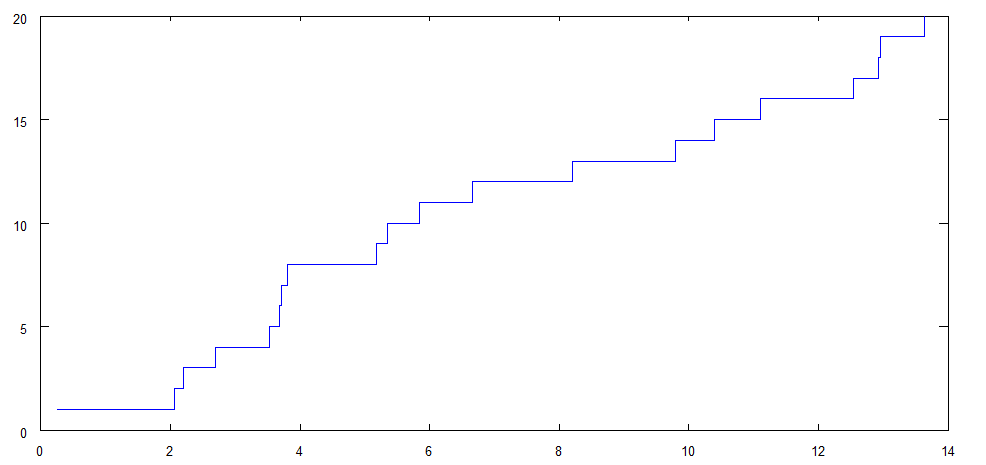
\includegraphics[width=0.7\textwidth]{4poisson1.png}
\caption{Poisson modo 1}
\label{Poisson modo 1}
\end{figure}
Para el segundo c\'odigo simulamos una v.a. $Poi(\lambda)$; con esto condicionamos a que al tiempo $t$ ocurra tal cantidad de saltos. Despu\'es se simulan v.a. uniformes sobre $[0,t]$ y se ordenan, indicando los puntos donde $N$ tendr� los saltos.
\begin{lstlisting}
t=30;
l=.7;
n=poissrnd(t*l);
T=zeros(1,n);
T=unifrnd(0,20,1,n);
T=sort(T);
N=1:n;
[Ts, Ns] = stairs (T, N );
plot(Ts,Ns)
\end{lstlisting}

Una realizaci\'on de este c\'odigo se encuentra en la Figura \ref{Poisson modo 2}.

\begin{figure}
\centering
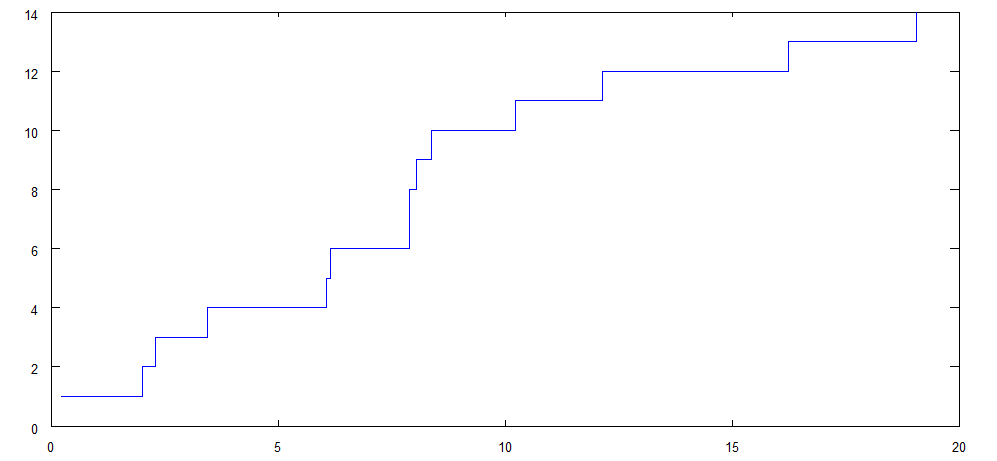
\includegraphics[width=0.7\textwidth]{5poisson2.png}
\caption{Poisson modo 2}
\label{Poisson modo 2}
\end{figure}

Nota: En un principio cre\'i que se ped\'ia $\lambda\in (0,1)$, no el proceso $N$ en $[0,1]$. Cuando v\'i mi error, ya hab\'ia cerrado Octave y ya ten\'ia todo listo para integrar la prueba a LATEX; siento la modificaci\'on que le hice al ejercicio, pero basta con cambiar en el c\'odigo a una $\lambda$ mayor (para que haya m\'as saltos y los podamos notar) y hacer $t=1$ en el segundo modelo, y para el primero meter un ciclo de simulaci\'on de v.a. $Exp(\lambda)$ (e irlas sumando) hasta que el proceso haya superado el tiempo $1$, y entonces tomarlo hasta el paso anterior.
\end{proof}
\end{enumerate}
\end{problema}
\begin{problema}
%Simulaci\'on de un proceso Poisson puntual... subordinador...
 Sea $\Xi$ una medida de Poisson aleatoria en $(0,\infty)\times (0,\infty)$ cuya medida de intensidad $\nu$ est\'a dada por $\imf{\nu}{ds,dx}=\indi{x>0}C/x^{1+\alpha}\, ds\,dx$. 
 \begin{enumerate}
\item Determine los valores de $\alpha$ para los cuales $\int 1\wedge x\,\imf{\nu}{dx}<\infty$. 
\begin{proof}
Se tomar\'a $\nu (\dd s, \dd x)=\mathds{1}_{s\ge 0, x> 0} C/x^{1+\alpha}\dd s \dd x$. Para $s<0$ cualquier integral ser\'a exactamente igual a $0$. Por lo tanto, elijamos $s\ge 0$. Entonces,
\begin{align*}
\int 1\wedge x \nu (s,\dd s) & = \int (1\wedge x) \mathds{1}_{s\ge 0, x> 0} \frac{C}{x^{1+\alpha}}\dd x\\
& =\int_0^\infty (1\wedge x)  \frac{C}{x^{1+\alpha}}\dd x\\
& =\int_0^1 x  \frac{C}{x^{1+\alpha}}\dd x + \int_1^\infty 1  \frac{C}{x^{1+\alpha}}\dd x\\
& =\int_0^1 \frac{C}{x^{\alpha}}\dd x + \int_1^\infty  \frac{C}{x^{1+\alpha}}\dd x.
\end{align*}
Estudiemos estas dos integrales a continuaci\'on. Si $\alpha=1$, entonces
\[\int_0^1 \frac{C}{x^{\alpha}}\dd x = [C\log (x)]_0^1 = -C \lim_{x\to 0}\log(x) ,\]
que converge a $\infty$ y por lo tanto no es un valor posible. Supongamos que $\alpha\neq 1$. Entonces
\begin{align*}
\int_0^1 \frac{C}{x^{\alpha}}\dd x & = \int_0^1 C x^{-\alpha}\dd x\\
& = \left[\frac{C x^{1 -\alpha}}{1 -\alpha}\right]_0^1 = \frac{C}{1 -\alpha} - \lim_{x\to 0}\frac{C x^{1 -\alpha}}{1 -\alpha},
\end{align*}
de manera que esta integral existe (y es igual a $C/(1-\alpha )$) si y solo si $\alpha < 1$.

Por otro lado, si $\alpha = 0$,
\[\int_1^\infty  \frac{C}{x}\dd x = C\log_{x\to\infty} \log (x),\]
el cual converge a $\infty$ y tamoco es una valor posible. Por lo tanto, supongamos que $\alpha\neq 0$. Entonces
\begin{align*}
\int_1^\infty  \frac{C}{x^{1+\alpha}}\dd x & = \int_1^\infty  C x^{-(1+\alpha )}\dd x = \left[\frac{C x^{-\alpha}}{-\alpha}\right]_1^\infty\\
& = \lim_{x\to\infty} \frac{C x^{-\alpha}}{-\alpha} + \frac{C}{\alpha},
\end{align*}
de manera que la integral existe (y es igual a $C/\alpha$ si y solo si $\alpha >0$. 

Por lo tanto, la integral a investigar es finita si y solo si $\alpha\in (0,1)$.
\end{proof}
 \end{enumerate}
Nos restringimos ahora a valores de $\alpha$ para los cuales la integral anterior sea finita. Sean $\imf{f_t}{s,x}=\indi{s\leq t}x$ y $X_t=\Xi f_t$. 
 \begin{enumerate}[resume]
 \item Determine los valores  de $\alpha$ para los cuales $X_t<\infty$ para toda $t\geq 0$ casi seguramente.
 \begin{proof}
 En clase se demostr\'o que $\Xi f_t$ es finito c.s. si y s\'olo si $\int (1\wedge f_t) \dd \nu$ es finito. Entonces,
 \begin{align*}
 \int (1\wedge f_t) \dd \nu & = \int \int (1\wedge \mathds{1}_{s\ge t} x) \mathds{1}_{s\ge 0, x> 0}\frac{C}{x^{1+\alpha}}\dd x\dd s\\
 & = \int_0^t \int_0^\infty (1\wedge x) \frac{C}{x^{1+\alpha}}\dd x\dd s\\
 & = \int_0^t  \left( \int_0^1 \frac{C}{x^{\alpha}}\dd x + \int_1^\infty  \frac{C}{x^{1+\alpha}}\dd x\right)\dd s\\
  & = \int_0^t  \left( \frac{C}{1-\alpha} + \frac{C}{\alpha}\right)\dd s\nota{(Por inciso anterior)}\\
  & = t\left( \frac{C}{1-\alpha} + \frac{C}{\alpha}\right) = \frac{C t}{\alpha (1-\alpha)}.
 \end{align*}
 En conclusi\'on, la restricci\'on $\alpha \in (0,1)$ es necesaria y suficiente.
 \end{proof}
 \end{enumerate}
 Nos restringiremos a dichos valores de $\alpha$. 
 \begin{enumerate}[resume]
 \item Calcule $\esp{e^{-\lambda X_t}}$ y pruebe que $X_{t}$ tiene la misma distribuci\'on que $t^{1/\alpha}X_1$. 
 \begin{proof}
Por clase, sabemos que
\begin{align*}
\mean (e^{-\lambda X_t}) & = \mean (e^{-\Xi [\lambda f_t]})\nota{($\Xi$ es un operador lineal)}\\
& = \exp (-\int (1-e^{-\lambda f_t})\dd \nu).
\end{align*}
Calculando la integral,
\begin{align*}
\int (1-e^{-\lambda f_t})\dd \nu & = \int\int (1 - e^{-\lambda \mathds{1}_{s\le t}x})\mathds{1}_{s\ge 0, x > 0}\frac{C}{x^{1+\alpha}}\dd s \dd x\\
& = \int_0^\infty \int_0^t (1 - e^{-\lambda x})\frac{C}{x^{1+\alpha}}\dd s \dd x\\
& = Ct \int_0^\infty \frac{1 - e^{-\lambda x}}{x^{1+\alpha}} \dd x\\
& = Ct \int_0^\infty \frac{\int_0^x \lambda e^{-\lambda r}\dd r}{x^{1+\alpha}} \dd x\\
& = Ct\lambda \int_0^\infty \int_r^\infty \frac{e^{-\lambda r}}{x^{1+\alpha}}\dd x \dd r\\
& = Ct\lambda \int_0^\infty e^{-\lambda r} \left[\frac{1}{-\alpha x^\alpha}\right]_r^\infty \dd r\\
& = \frac{Ct\lambda }{\alpha}\int_0^\infty  \frac{e^{-\lambda r}}{ r^\alpha}\dd r\\
& = \frac{Ct\lambda }{\alpha}\frac{\lambda^\alpha}{\lambda}\int_0^\infty  \frac{e^{-\lambda r}}{ (\lambda r)^\alpha}\lambda \dd r\nota{(Multiplicando por un $1$ conveniente)}\\
& = \frac{Ct\lambda^{\alpha}}{\alpha}\int_0^\infty   (\lambda r)^{(-\alpha + 1) - 1} e^{-\lambda r}\dd (\lambda r)\\
& = \frac{Ct\lambda^{\alpha}}{\alpha} \Gamma (1-\alpha ),
\end{align*}
y por lo tanto,
\[\mean (e^{-\lambda X_t}) = \exp \left( - \frac{C t \lambda^\alpha \Gamma (1-\alpha )}{\alpha}\right),\]
que justamente corresponde a su transformada de Laplace.
Tomando $t=1$ y $\lambda = \lambda' t'^{1/\alpha}$, entonces
\[\mean (\exp ( -\lambda' t'^{1/\alpha} X_1 )) = \exp \left( - \frac{C \cdot 1\cdot (-\lambda' t'^{1/\alpha})^\alpha \Gamma (1-\alpha )}{\alpha}\right) = \exp \left( - \frac{C t' \lambda'^\alpha \Gamma (1-\alpha )}{\alpha}\right),\]
es decir $\mean (\exp (-\lambda (t^{1/\alpha}X_1))) = \mean (\exp (-\lambda X_t))$, es decir, sus transformadas de Laplace coinciden, y como son variables aleatorias no negativas c.s., \'estas deben tener la misma distribuci\'on.
 \end{proof}

\item Diga por qu\'e el siguiente c\'odigo en Octave simula la trayectoria aproximada del proceso $X$ en el intervalo $[0,1]$.
\begin{lstlisting}
C=1;
e=.000001;
alpha=1/2;
lambda=C/e^alpha;
T=1;
N=poissrnd(lambda*T, 1);
u=T*rand(N,1);
dx=e./rand(N,1).^(1/(alpha));
s=[0;cumsum(dx)];
t=[0;sort(u)];
subplot(1,2,1)
plot(t(2:length(t)),dx)
subplot(1,2,2)
plot(t,s)
\end{lstlisting}
\begin{proof}
Una realizaci\'on del c\'odigo anterior est\'a en la Figura \ref{Subordinador}.
\begin{figure}
\centering
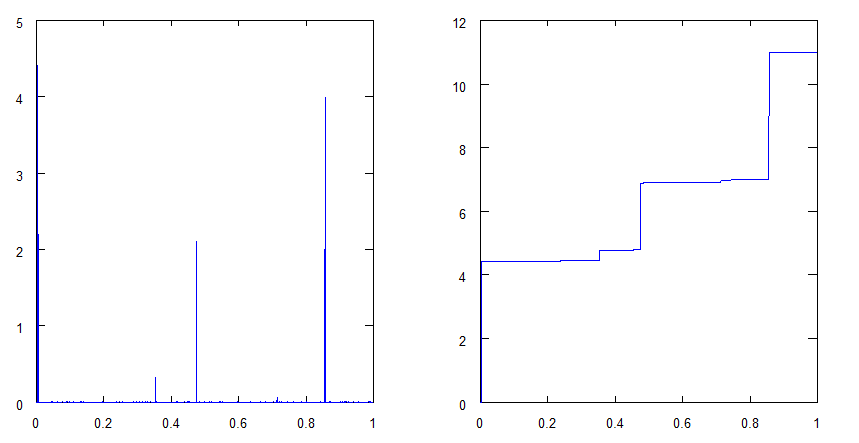
\includegraphics[width=0.7\textwidth]{6subord.png}
\caption{Subordinador}
\label{Subordinador}
\end{figure}
Lo que el c�digo hace es primero ubicar los puntos donde habr\'a saltos, para despu\'es decidir el tama�o de estos saltos, los cuales pueden ser chicos o grandes. Sin embargo, los saltos ser\'an de un tama�o m\'inimo de $.000001$.
\end{proof}
\end{enumerate}
\end{problema}

\begin{problema}
Pruebe que si $X$ tiene incrementos independientes entonces el proceso $X^t$ dado por $X^t_s=X_{t+s}-X_t$ es independiente de $\F^X_t=\sag{X_s:s\geq 0}$.
\begin{proof}
Supongamos que $X^t$ tiene incrementos independientes. La $\sigma$-\'algebra $\F_t=\sigma (X_s, 0\le s\le t)$ es generada por los subconjuntos de la forma
\[\{\omega\in\Omega : X_s (\omega )\in A \}\]
para todo $s\in [0,t]$ y $A\in\borr$. M\'as a\'un, $\F_t$ tambi\'en es generada por los subconjuntos de la forma 
\[\{X_{s_0}\in A_0, X_{s_1} - X_{s_0}\in A_1,\dots , X_{s_n} - X_{s_{n-1}}\in A_n \}\]
para todo $n\in\nats$, $0\le s_0 < s_1 <\dots <s_n\le t$ y $A_0,\dots ,A_n\in\borr$. Para ver esto, notemos que los subconjuntos del primer tipo se pueden ver como subconjuntos del segundo tipo si hacemos $A_1,\dots,A_n= \reals$. Ademas, los conjuntos del segundo tipo son $\F_t$-medibles y por lo tanto, generan justamente a $\F_t$. Llamaremos a la familia de subconjuntos del segundo tipo (uniendo al elemento $\{\emptyset\}$) como $\Cp_t$. Por la discusi\'on anterior se tendr\'a que $\sigma (\Cp_t )=\F_t$; adem\'as, notemos que $\Cp_t$ es un $\pi$-sistema.

Lo mismo se puede concluir para $\F^t=\sigma (X_r^t, r\ge 0) = \sigma (X_{t+r} - X_t, r\ge 0)$; es decir, que $\F^t$ es generada por subconjuntos de la forma
\[\{X_{t+r_0}- X_t \in B_0, X_{t+r_1} - X_{t+r_0}\in B_1, \dots, X_{t+r_m} - X_{t+r_{m-1}}\in B_m\}\]
para todo $m\in\nats$, $0\le r_0 < r_1 <\dots <r_m\le t$ y $B_0,\dots ,B_m\in\borr$. A la familia de subconjuntos de este tipo (uni\'on el elemento $\{\emptyset\}$) le llamaremos $\Cp^t$, donde tambi\'en se tendr\'a que $\sigma (\Cp^t )=\F^t$ y que $\Cp^t$ es un $\pi$-sistema.

Sea $D_0\in\Cp^t$ fijo, es decir,
\[D_0=\{X_{t+r_0^0}- X_t \in B_0^0, X_{t+r_1^0} - X_{t+r_0^0}\in B_1^0, \dots, X_{t+r_{m^0}^0} - X_{t+r_{m^0-1}^0}\in B_{m^0}\}.\]
para alg\'un $m^0\in\nats$, $0\le r_0^0 < r_1^0 <\dots <r_{m^0}^0\le t$ y $B_0^0,\dots ,B_{m^0}^0\in\borr$.
Definamos
\[\Ll_t := \{C\in\sigma (\Cp_t )=\F_t: \p (C\cap D_0 ) = \p(C)\p(D_0)\}.\]
Sea $C_0\in\Cp_t$, es decir,
\[C_0=\{X_{s_0^0} \in A_0^0, X_{s_1^0} - X_{s_0^0}\in A_1^0,\dots , X_{s_{n^0}^0} - X_{s_{n^0-1}^0}\in A_{n^0}^0\}\]
para alg\'un $n^0\in\nats$, $0\le s_0 < s_1 <\dots <s_{n^0}\le t$ y $A_0,\dots ,A_{n^0}\in\borr$.
Entonces
\begin{align*}
\p(C_0\cap D_0) & = \p(\{X_{s_0^0} \in A_0^0, X_{s_1^0} - X_{s_0^0}\in A_1^0,\dots , X_{s_{n^0}^0} - X_{s_{n^0-1}^0}\in A_{n^0}^0\}\cap\\
&\tres \{X_{t+r_0^0}- X_t \in B_0^0, X_{t+r_1^0} - X_{t+r_0^0}\in B_1^0, \dots, X_{t+r_{m^0}^0} - X_{t+r_{m^0-1}^0}\in B_{m^0}\})\\
& = \p(\{X_{s_0^0} \in A_0^0, X_{s_1^0} - X_{s_0^0}\in A_1^0,\dots , X_{s_{n^0}^0} - X_{s_{n^0-1}^0}\in A_{n^0}^0\}\cap\\
&\tres \{X_t-X_{s_{n^0}^0}\in\reals\}\cap\\
&\tres \{X_{t+r_0^0}- X_t \in B_0^0, X_{t+r_1^0} - X_{t+r_0^0}\in B_1^0, \dots, X_{t+r_{m^0}^0} - X_{t+r_{m^0-1}^0}\in B_{m^0}\})\\
& = \p(X_{s_0^0} \in A_0^0, X_{s_1^0} - X_{s_0^0}\in A_1^0,\dots , X_{s_{n^0}^0} - X_{s_{n^0-1}^0}\in A_{n^0}^0)\times\\
&\tres \prob(X_t-X_{s_{n^0}^0}\in\reals )\times\\
&\tres \p (X_{t+r_0^0}- X_t \in B_0^0, X_{t+r_1^0} - X_{t+r_0^0}\in B_1^0, \dots, X_{t+r_{m^0}^0} - X_{t+r_{m^0-1}^0}\in B_{m^0})\\
& =\p (C_0)\times 1 \times\p (D_0),
\end{align*}
de manera que $\Cp_t\subset\Ll_t$. Si demostramos que $\Ll_t$ es un $\lambda$-sistema, se tendr\'ia que $\Ll_t=\sigma (\Cp_t )$; esta prueba es muy sencilla y se ha realizado en repetidas ocasiones; esta vez bastar\'a con utilizar la propiedad de aditividad finita continuidad de la funci\'on de probabilidad, sin embargo, la demostraci\'on formal ser\'a omitida.
A continuaci\'on, tomemos un $C_0'\in \F_t$ fijo. Definamos
\[\Ll^t:=\{D\in \sigma (\Cp^t)=\F_t : \p (C_0'\cap D) = \p(C_0')\p(D)\}.\]
Por el resultado anterior, se tiene que $\Cp^t\subset\Ll^t$ y de igual manera, se omite la prueba de que $\Ll^t$ es un $\lambda$-sistema (es pr\'acticamente la misma). As\'i pues, se concluye que $\Ll_2 = \sigma (\Cp^t ) = \F^t$, lo que quiere decir que para todo $C\in\F_t$ y $D\in\F^t$, se tiene que $\p(C\cap D) = \p (C) \p(D)$, es decir, $X^t$ es independiente de $\F_t$.
\end{proof}
Calcular la esperanza y varianza del proceso de Poisson y de Poisson compuesto (en t\'erminos de la intensidad y la distribuci\'on de salto). Probar que si $X$ es
\begin{esn}
\esp{e^{iu Z_t}}=e^{-\lambda t\paren{1-\imf{\psi}{u}}}\quad\text{donde}\quad \imf{\psi}{u}=\esp{e^{iu \xi_1}}. 
\end{esn}

\begin{proof}
Sea $N_t$ el proceso Poisson de intesidad $\lambda$. Entonces, como $N_t\sim Poi (\lambda t)$, se tiene que
\[\mean (N_t) = \sum_{i=1}^\infty i e^{\lambda t}\frac{(\lambda t)^i}{i!} = \sum_{i=0}^\infty i e^{\lambda t}\frac{(\lambda t)^{i+1}}{i!} = \lambda t.\]
De la misma manera,
\begin{align*}
\mean(N_t^2) & =\sum_{i=1}^\infty i^2 e^{\lambda t}\frac{(\lambda t)^i}{i!}=\sum_{i=1}^\infty i e^{\lambda t}\frac{(\lambda t)^i}{i-1!}\\
& = \sum_{i=0}^\infty (i+1) e^{\lambda t}\frac{(\lambda t)^{i+1}}{i!}\\
& = (\lambda t)\mean (N_t) + (\lambda t) = (\lambda t)^2 + (\lambda t),
\end{align*}
y por lo tanto
\[Var(N_t) = \mean (N_t^2) - \mean (N_t)^2 = (\lambda t)^2 + (\lambda t) - (\lambda t)^2 = \lambda t.\]
Sea $Z_t$ el proceso Poisson compuesto con saltos $\{\xi_i\}_i\in\nats$ independientes e id\'enticamente distribuidos, es decir,
\[Z_t = \sum_{i=1}^{N_t} \xi_i.\]
Entonces
\begin{align*}
\mean (Z_t) & = \mean \left(\sum_{i=1}^{N_t}\xi_i \right) = \mean \left(\sum_{i=1}^{\infty} \xi_i\mathds{1}_{T_i\le t}\right)\\
& = \sum_{i=1}^{\infty} \mean \left(\xi_i\mathds{1}_{T_i\le t}\right) = \sum_{i=1}^{\infty} \mean (\xi_i)\mean \left(\mathds{1}_{T_i\le t}\right)\nota{(Por independencia)}\\
& = \sum_{i=1}^{\infty} \mean (\xi_1)\mean \left(\mathds{1}_{T_i\le t}\right)\nota{(Las $\xi_i$'s son v.a.i.i.d.)}\\
& = \mean(\xi_1) \sum_{i=1}^{\infty} \mean \left(\mathds{1}_{T_i\le t}\right) = \mean(\xi_1) \mean \left(\sum_{i=1}^{\infty}\mathds{1}_{T_i\le t}\right)\\
& = \mean(\xi_1) \mean \left(N_t\right) = \mean(\xi_1)(\lambda t).
\end{align*}
Para calcular su varianza,
\begin{align*}
\mean (Z_t^2) & = \mean\left(\mean\left(Z_t^2|N_t\right)\right)\\
& = \mean\left(\mean\left(\left(\sum_{i=1}^{N_t} \xi_i\right)^2 | N_t\right)\right)\\
& = \mean\left(\mean\left(\sum_{j=0}^{\infty}\mathds{1}_{N_t = j}\left(\sum_{i=1}^{j} \xi_i\right)^2 | N_t\right)\right)\\
& = \mean\left(\sum_{j=0}^{\infty}\mathds{1}_{N_t = j} \mean\left(\left(\sum_{i=1}^{j} \xi_i\right)^2 | N_t\right)\right)\nota{(Por medibilidad y Fubini)}\\
& = \mean\left(\sum_{j=0}^{\infty}\mathds{1}_{N_t = j} \mean\left(\left(\sum_{i=1}^{j} \xi_i\right)^2 \right)\right)\nota{(Por independencia de los $\xi_i$'s con $N_t$)}\\
& = \mean\left(\sum_{j=0}^{\infty}\mathds{1}_{N_t = j} \left(Var \left(\sum_{i=1}^{j} \xi_i\right) + \mean \left(\sum_{i=1}^{j} \xi_i\right)^2 \right)\right)\\
& = \mean\left(\sum_{j=0}^{\infty}\mathds{1}_{N_t = j} \left(j\times Var \left( \xi_1\right) + j^2\times\mean \left(\xi_1\right)^2 \right)\right)\nota{(Por que las $\xi_i$'s son v.a.i.d.d.)}\\
& = \mean\left(N_t\times Var \left( \xi_1\right) + N_t^2\times\mean \left(\xi_1\right)^2 \right)\\
& = \mean (N_t) Var \left( \xi_1\right) + \mean (N_t^2)\mean \left(\xi_1\right)^2\\
& = \mean (N_t) Var \left( \xi_1\right) + (Var(N_t) + \mean (N_t^2))\mean \left(\xi_1\right)^2\\
& = (\lambda t) Var \left( \xi_1\right) + (\lambda t)\mean \left(\xi_1\right)^2 + (\mean (N_t)\mean \left(\xi_1\right))^2\\
& = (\lambda t) (\mean(\xi_1^2)) + (\mean (N_t)\mean \left(\xi_1\right))^2,
\end{align*}
y por lo tanto,
\[Var (Z_t) = \mean (Z_t^2) - \mean (Z_t)^2 = (\lambda t) (\mean(\xi_1^2)).\]

Para calcular $\mean (e^{i u Z_t})$, se sigue un procedimiento similar, de manera que
\begin{align*}
\mean (e^{i u Z_t}) & = \mean \left(\mean \left(\exp\left(i u \sum_{j=1}^{N_t}\xi_j\right) | N_t \right)\right)\\
& = \mean \left(\mean \left(\sum_{k=0}^\infty \mathds{1}_{N_t=k}\exp\left(i u \sum_{j=1}^{k}\xi_j\right) | N_t \right)\right)\\
& = \mean \left(\sum_{k=0}^\infty \mathds{1}_{N_t=k} \mean \left(\exp\left(i u \sum_{j=1}^{k}\xi_j\right) | N_t \right)\right)\\
&\tres\nota{(Medibilidad y Fubini)}\\
& = \mean \left(\sum_{k=0}^\infty \mathds{1}_{N_t=k} \mean \left(\exp\left(i u \sum_{j=1}^{k}\xi_j\right) \right)\right)\\
&\tres\nota{(Independencia con $N_t$)}\\
& = \mean \left(\sum_{k=0}^\infty \mathds{1}_{N_t=k} \mean \left(\exp\left(i u \xi_1\right) \right)^k\right)\\
&\tres\nota{(Las $\xi_j$'s son v.a.i.i.d.)}\\
& = \mean \left( \mean \left(\exp\left(i u \xi_1\right) \right)^{N_t}\right) = \mean(\psi (u)^{N_t})\\
& = \sum_{i=0}^\infty \psi (u)^i \times e^{-\lambda t}\frac{(\lambda t)^i}{i!}\\
& = e^{-\lambda t} \sum_{i=0}^\infty  \frac{(\psi (u)\lambda t)^i}{i!}\\
& = e^{-\lambda t} e^{\psi (u)\lambda t} = e^{-\lambda t( 1 - \psi (u))}
\end{align*}
\end{proof}


Sea $N$ un proceso de L\'evy tal que $N_t$ tiene distribuci\'on de par\'ametro $\lambda t$. 
\begin{enumerate}
\item Pruebe que casi seguramente las trayectorias de $N$ son no-decrecientes.
\begin{proof}
Tendr\'iamos que probar que para todo $s,t\ge 0$, $N_{t+s} - N_t \ge 0$. Sin embargo, esto es directo al utilizar los incrementos estacionarios del proceso de Levy, ya que tenemos que $N_{t+s} - N_t$ es igual en distribuci\'on a $N_s\sim Poi(\lambda )$, la cual toma valores en $\entpos$ con probabilidad 1, demostrando entonces que $N_{t+s} - N_t\ge 0$.
Adem\'as, este proceso $N$ que toma valores en una cantidad numerable de estados ($\entpos$) y que es no decreciente, debe tener trayectorias constante a pedazos. Notemos que lo �nico que falta para afirmar que \'este es un proceso Poisson, es que sus incrementos sean de una unidad en una unidad, pero esa es la finalidad de los siguientes incisos.
\end{proof}

\item Sea $\Xi$ la \'unica medida en $\mc{B}_{\re_+}$ tal que $\imf{\Xi}{[0,t]}=N_t$. Pruebe que $\Xi$ es una medida de Poisson aleatoria de intensidad $\lambda \cdot\leb$.
\begin{proof}
La prueba de este inciso es exactamente la misma que la de la Proposici\'on 4.5 (p\'ag 105); en tal prueba se hace la suposici\'on de que $N$ s un proceso Poisson (cosa que no tenemos como hip\'otesis) sin embargo, las \'unicas propiedades que se utiliza para tal demostraci\'on son los incrementos independientes y estacionarios (que tenemos porque $N$ es un proceso de Levy), que $N_t\sim Poi(\lambda )$ y que las trayectorias son crecientes y constantes a pedazos (que tenemos por la discusi\'on del inciso anterior). Dicha prueba ser\'a omitida en esta tarea por que b\'asicamente ser\'ia una copia de la que se encuentra en las notas (con el intercambio de las palabras 'proceso Poisson' por la propiedad que se est\'e utilizando de las mencionadas anteriormente).
\end{proof}

\item Concluya que $N$ es un proceso de Poisson de intensidad $\lambda$.
\begin{proof}
En la p\'ag 108 de las notas, se demuestra que cualquier medida de Poisson aleatoria $\Xi\in\reals_+$ con intensidad $\lambda\times Leb$ corresponde a un proceso de Poisson. Por lo tanto, ya que se demostro que la medida $\Xi$ en el anterior inciso cumple con tales propiedades, debe de suceder que $N$ es un proceso Poisson.
\end{proof}
\end{enumerate}
\end{problema}

\begin{problema}
Sea $P_t$ la probabilidad de transici\'on en $t$ unidades de tiempo para el proceso de Poisson de par\'ametro $\lambda$. 

Al utilizar el teorema del biniomio, pruebe directamente que las probabilidades de transici\'on del proceso de Poisson satisfacen las ecuaciones de Chapman-Kolmogorov $P_{t+s}=P_tP_s$. D\'e adem\'as un argumento probabil\'istico, basado en condicionar con lo que sucede al tiempo $s$, para probar dicha ecuaci\'on. 

Sea\begin{esn}
\imf{Q}{i,j}=\begin{cases}
-\lambda&j=i\\
\lambda&j=i+1\\
0&j\neq i,i+1
\end{cases}.
\end{esn}Pruebe directamente que se satisfacen las ecuaciones de Kolmogorov\begin{equation*}
%\label{CKEquationsForPoisson}
\frac{d}{dt}\imf{P_t}{i,j}=\imf{QP_t}{i,j}=\imf{P_tQ}{i,j},
\end{equation*}donde $QP_t$ es el producto de las matrices $Q$ y $P_t$.
\end{problema}
\begin{proof}
Elijamos $i,j\in\nats$. Sabemos que
\[P_r(i,j) = \prob (N_r = j-i) = e^{-\lambda r}\frac{(\lambda r)^{j-i}}{(j-i)!}\]
cuando $i\le j$ y $0$ en otro caso. Sea entonces $i\le j$.
Entonces,
\begin{align*}
P_{t+s} (i,j) & = e^{-\lambda (t+s)}\frac{(\lambda (t+s))^{j-i}}{(j-i)!}\\
& = e^{-\lambda (t+s)}\frac{\sum_{l=0}^{j-i} {j-i \choose {l}} t^l s^{j-i-l}}{(j-i)!}\\
& = e^{-\lambda (t+s)}\sum_{l=0}^{j-i} \frac{t^l s^{j-i-l}}{l! (j-i-l)!}.
\end{align*}
Si multiplicamos las matrices $P_t$ y $P_s$, tendr\'iamos que
\begin{align}
(P_t P_s) (i,j) & = \sum_{l=0}^\infty P_t(i,l) P_s(l,j)\label{eq:chapkol1}\\
& = \sum_{l=i}^j P_t(i,l) P_s(l,j)\nonumber\\
& \tres\nota{(Se tiene que $P_t(i,l)=P_s(l,j)=0$ para todo $l<i$ y $j<l$)}\nonumber\\
& = \sum_{l=i}^j e^{-\lambda t}\frac{(\lambda t)^{l-i}}{(l-i)!}\times e^{-\lambda s}\frac{(\lambda s)^{j-l}}{(j-l)!}\nonumber\\
& = e^{-\lambda (t+s)}\lambda^{j-i} \sum_{l=i}^j \frac{t^{l-i}s^{j-l}}{(l-i)!(j-l)!}\nonumber\\
& = e^{-\lambda (t+s)}\lambda^{j-i} \sum_{l'=0}^{j-1} \frac{t^{l'}s^{j-i-l'}}{l'!(j-i-l')!}\nota{(Haciendo $l'=l-i$)}.\nonumber
\end{align}
Notemos que en el caso $i>j$, los sumandos de (\ref{eq:chapkol1}) son exactamente igual a 0, ya que para todo $l$, se tendr\'a que $i>l$ o que $j<l$, y en cualquier caso la multiplicaci\'on de probabilidades se anula. Por lo tanto se ha comprobado que las entradas $(i,j)$ para todo $i,j\in\nats$ de las matrices $P_{t+s}$ y $P_t P_s$ coinciden y por lo tanto, son id\'enticas.
Probabilisticamente, de nuevo fijandonos s\'olo en el caso $i\le j$ (el caso $i>j$ da como resultado probabilidades nulas), se tiene que
\begin{align*}
P_{t+s}(i,j)& =\p(N_{t+s} = j-i)\\
& = \sum_{l=0}^{j-i}\p(N_{t+s} = j-i, N_t = l)\\
& = \sum_{l=0}^{j-i}\p(N_{t+s} - N_t= j-(i+l), N_t = l)\\
& = \sum_{l=0}^{j-i}\p(N_{t+s} - N_t= j-(i+l))\p( N_t = l)\nota{(Por incr. ind.)}\\
& = \sum_{l=0}^{j-i}P_s(i+l,j)P_t(0,l)\\
& = \sum_{l=0}^{j-i}P_s(i+l,j)P_t(i,i+l)\\
& = \sum_{l'=i}^{j}P_s(l',j)P_t(i,l')\nota{(Haciendo $l'=l+i$)}\\
= (P_tP_s)(i,j),
\end{align*}
demostrando las ecuaciones de Chapman-Kolmogorov para el proceso Poisson. Para demostrar las ecuaciones diferenciales de Kolmogorov, veamos que para todo $i\le j$
\begin{align*}
\deror{r}P_r(i,j) & = \deror{r} e^{-\lambda r}\frac{(\lambda r)^{j-i}}{(j-i)!}\\
&  = e^{-\lambda r}\frac{\lambda^{j-i}}{(j-i)!}(j-i) r^{j-i-1} -\lambda e^{-\lambda r}\frac{(\lambda r)^{j-i}}{(j-i)!}\\
& = \lambda\left( e^{-\lambda r}\frac{(\lambda r)^{j-(i+1)}}{(j-(i+1))!}\right) - \lambda e^{-\lambda r}\frac{(\lambda r)^{j-i}}{(j-i)!}\\
& = \lambda P_r(i+1,j) - \lambda P_r(i,j).
\end{align*}
Por otro lado,
\begin{align*}
(QP_r)(i,j)& =\sum_{l=0}^\infty Q(i,l) P_r(l,j)\\
& = Q(i,i)P_r(i,j) + Q(i,i+1)P_r(i+1,j)\\
& =  - \lambda P_r(i,j) + \lambda P_r(i+1,j).
\end{align*}
Adem\'as,
\begin{align}
(P_r Q)(i,j)& =\sum_{l=0}^\infty P_r(i,l) Q(l,j)\label{eq:chapkol2}\\
& = P_r(i,j)Q(j,j) + P_r(i,j-1)Q(j-1,j)\nonumber\\
& =  - \lambda P_r(i,j) + \lambda P_r(i,j-1)\nonumber\\
& =  - \lambda P_r(i,j) + \lambda P_r(i+1,j).\nonumber
\end{align}
Nuevamente, el caso $j<i$ da probabilidades nulas en todas las sumas (\ref{eq:chapkol2}), lo cual tiene sentido ya que estamos derivando una probabilidad constante (cero). Por lo tanto, se tendr\'a que
\[\deror{r} P_r = QP_r=P_rQ.\]
\end{proof}

\begin{problema}[Tomado del examen general de probabilidad del Posgrado en Ciencias Matem\'aticas, UNAM, \href{http://www.posgradomatematicas.unam.mx/contenidoEstatico/archivo/files/pdf/Examenes_Generales/Probabilidad/Probabilidad2011-1.pdf}{Febrero 2011}]
Una planta de producci\'on toma su energ\'ia de dos generadores. La cantidad de generadores al tiempo $t$ est\'a representado por una cadena de Markov a tiempo continuo $\set{X_t,t\geq 0}$ con espacio de estados $E=\set{0,1,2}$ y matriz infinit\'esimal $Q$ dada por\begin{esn}
Q=\begin{pmatrix}
-6&6&0\\
1&-7&6\\
0&2&-2
\end{pmatrix}.
\end{esn}
\begin{enumerate}
\item Encuentre la matriz de transici\'on de la cadena de Markov de los estados distintos que toma $X$, clasifique los estados, diga si existe una \'unica distribuci\'on invariante y en caso afirmativo, encu\'entrela. Calcule expl\'icitamente las potencias de la matriz de transici\'on. (Recuerde que de ser posible diagonalizar, esta es una buena estrategia.)
\begin{proof}
Notemos que no hay ningun estado absorbente, por lo tanto,
\[P(i,j) = \frac{Q(i,j)}{c(i)}(1-\delta_{ij}),\]
es decir,
\[P=\begin{pmatrix}
0 & 1 & 0 \\ 
1/7 & 0 & 6/7 \\ 
0 & 1 & 0
\end{pmatrix}.\]

Es claro que la trayectoria $0 \to 1\to 2 \to 1 \to 0$ es v\'alida, y por lo tanto todos los estados se comunican y el proceso ser\'a irreducible. Al tener un n\'umero finito de estados, ser\'a recurrente positiva y por lo tanto existir\'a una distribuci\'on estacionaria $\nu=(\nu_1,\nu_2,\nu_3)$ que resuelva el sistema
\[\nu P = \nu,\]
es decir, querems resolver el sistema
\[ \begin{pmatrix}
\nu_1 & \nu_2 & \nu_3
\end{pmatrix} = \begin{pmatrix}
\nu_1 & \nu_2 & \nu_3
\end{pmatrix} \begin{pmatrix}
0 & 1 & 0 \\ 
1/7 & 0 & 6/7 \\ 
0 & 1 & 0
\end{pmatrix} = \begin{pmatrix}
\nu_2 /7 & \nu_1 + \nu_3 & 6 \nu_2 / 7
\end{pmatrix}. \]
Fijando $\nu_2=7$, se tiene que $(\nu_1,\nu_2,\nu_3) = (1,7,6)$, y normalizando para que $\nu_1 + \nu_2 + \nu_3 =1$, tendremos que $(1/14, 1/2, 3/7)$ es la distribuci\'on invariante.

Para calcular las potencias de $P$, haremos una diagonalizaci\'on. Entonces

\[\det{\begin{pmatrix}
-6-\lambda &6&0\\
1&-7-\lambda &6\\
0&2&-2-\lambda
\end{pmatrix}} = -\lambda (\lambda + 1)(\lambda -1),\]
es decir, sus eigenvalores ser\'an $0, -1$ y $1$.

Para $\lambda_1=0$, el sistema
\[\begin{pmatrix}
0 \\ 
0 \\ 
0
\end{pmatrix} = \begin{pmatrix}
0 & 1 & 0 \\ 
1/7 & 0 & 6/7 \\ 
0 & 1 & 0
\end{pmatrix} \begin{pmatrix}
x_1 \\ 
x_2 \\ 
x_3
\end{pmatrix} = \begin{pmatrix}
x_2 \\ 
x_1/7 + 6 x_3 /7 \\ 
x_2
\end{pmatrix} \]
tiene como soluci\'on al vector $(6, 0 , -1)^T$.

Para $\lambda_2=-1$, el sistema
\[\begin{pmatrix}
0 \\ 
0 \\ 
0
\end{pmatrix} = \begin{pmatrix}
-1 & 1 & 0 \\ 
1/7 & -1 & 6/7 \\ 
0 & 1 & -1
\end{pmatrix} \begin{pmatrix}
y_1 \\ 
y_2 \\ 
y_3
\end{pmatrix} = \begin{pmatrix}
-y_1+y_2 \\ 
y_1/7 -y_2 + 6 y_3 /7 \\ 
y_2 - y_3
\end{pmatrix} \]
tiene como soluci\'on al vector $(1, 1 , 1)^T$.

Para $\lambda_3=1$, el sistema
\[\begin{pmatrix}
0 \\ 
0 \\ 
0
\end{pmatrix} = \begin{pmatrix}
1 & 1 & 0 \\ 
1/7 & 1 & 6/7 \\ 
0 & 1 & 1
\end{pmatrix} \begin{pmatrix}
z_1 \\ 
z_2 \\ 
z_3
\end{pmatrix} = \begin{pmatrix}
z_1+z_2 \\ 
z_1/7 +z_2 + 6 z_3 /7 \\ 
z_2 + z_3
\end{pmatrix} \]
tiene como soluci\'on al vector $(1, -1 , 1)^T$.
Entonces $P=A D A^{-1}$, donde
\[A=\begin{pmatrix}
6 & 1 & 1 \\ 
0 & 1 & -1 \\ 
-1 & 1 & 1
\end{pmatrix} \tres\mbox{ y } \tres D = \begin{pmatrix}
0 & 0 & 0 \\ 
0 & -1 & 0 \\ 
0 & 0 & 1
\end{pmatrix} .\]
Mediante el m\'etodo de Gauss (hecho en papel pero omitido en este archivo), es f\'acil concluir que
\[A^{-1}=\frac{1}{14}\begin{pmatrix}
2 & 0 & -2 \\ 
1 & 7 & 6 \\ 
1 & -7 & 6
\end{pmatrix},\] 
de manera que
\begin{align*}
P^n = AD^n A^{-1} & =\frac{1}{14} \begin{pmatrix}
6 & 1 & 1 \\ 
0 & 1 & -1 \\ 
-1 & 1 & 1
\end{pmatrix} \begin{pmatrix}
0 & 0 & 0 \\ 
0 & {-1}^n & 0 \\ 
0 & 0 & 1
\end{pmatrix}\begin{pmatrix}
2 & 0 & -2 \\ 
1 & 7 & 6 \\ 
1 & -7 & 6
\end{pmatrix}\\
& = \frac{1}{14}\begin{pmatrix}
(-1)^n + 1 & (-1)^n 7 - 7 & (-1)^n 6 + 6 \\ 
(-1)^n - 1 & (-1)^n 7 + 7 & (-1)^n 6 - 6 \\ 
(-1)^n + 1 & (-1)^n 7 - 7 & (-1)^n 6 + 6 \\ 
\end{pmatrix}.
\end{align*}
Notemos que varios de esos t\'erminos se eliminan si hacemos casos cuando $n$ es par o impar. De cualquier manera, es sencillo notar que esta matriz diverge, hecho que era claro al notar que la matriz de transici\'on $P$ no es aperi\'odica.
\end{proof}
\item ?`Cu\'al es la probabilidad de que ambos generadores est\'en trabajando al tiempo $t$ si s\'olo uno trabaja al tiempo cero? 
\begin{proof}
Necesitamos calcular $P_t$ de manera que se diagonalizar\'a la matriz $Q$. Entonces
\[\det{\begin{pmatrix}
-6&6&0\\
1&-7&6\\
0&2&-2
\end{pmatrix}} = -\lambda (\lambda + 5)(\lambda + 10),\]
por lo que sus eigenvalores son $0,-5$ y $-10$.

Para $\lambda_1=0$, el sistema
\[\begin{pmatrix}
0 \\ 
0 \\ 
0
\end{pmatrix} = \begin{pmatrix}
-6 & 6 & 0 \\ 
1 & -7 & 6 \\ 
0 & 2 & -2
\end{pmatrix} \begin{pmatrix}
x_1 \\ 
x_2 \\ 
x_3
\end{pmatrix} = \begin{pmatrix}
-6 x_1 + 6 x_2 \\ 
x_1 - 7 x_2 + 6 x_3 \\ 
2 x_2 - 2 x_3
\end{pmatrix} \]
tiene como soluci\'on al vector $(1,1,1)^T$.

Para $\lambda_2=-5$, notemos que el sistema
\[\begin{pmatrix}
0 \\ 
0 \\ 
0
\end{pmatrix} = \begin{pmatrix}
-1 & 6 & 0 \\ 
1 & -2 & 6 \\ 
0 & 2 & 3
\end{pmatrix} \begin{pmatrix}
y_1 \\ 
y_2 \\ 
y_3
\end{pmatrix} = \begin{pmatrix}
- y_1 + 6 y_2 \\ 
y_1 - 2 y_2 + 6 y_3 \\ 
2 y_2 +3 y_3
\end{pmatrix} \]
tiene como soluci\'on (al fijar $y_2=-3$) al vector $(-18, -3 2)$.

Para $\lambda_3=-10$, el sistema
\[\begin{pmatrix}
0 \\ 
0 \\ 
0
\end{pmatrix} = \begin{pmatrix}
4 & 6 & 0 \\ 
1 & 3 & 6 \\ 
0 & 2 & 8
\end{pmatrix} \begin{pmatrix}
z_1 \\ 
z_2 \\ 
z_3
\end{pmatrix} = \begin{pmatrix}
4 z_1 + 6 z_2 \\ 
z_1 +3 z_2 + 6 z_3 \\ 
2 z_2 +8 z_3
\end{pmatrix} \]
tiene como soluci\'on (al fijar $z_3 = 1$) al vector $(6,-4,1)^T$. 

Entonces $Q=A D A^{-1}$, donde
\[A=\begin{pmatrix}
1 & -18 & 6 \\ 
1 & -3 & -4 \\ 
1 & 2 & 1
\end{pmatrix} \tres\mbox{ y } \tres D = \begin{pmatrix}
0 & 0 & 0 \\ 
0 & -5 & 0 \\ 
0 & 0 & -10
\end{pmatrix} .\]
Usando el m\'etodo de Gauss, se tendr\'a que
\[A^{-1}=\frac{1}{25}\begin{pmatrix}
1 & 6 & 18 \\ 
-1 & -1 & 2 \\ 
1 & -4 & 3
\end{pmatrix}.\]
Entonces
\begin{align*}
P_t & = e^{Qt} = \sum_{n=0}^\infty\frac{ Q^n t^n}{n!} = \sum_{n=0}^\infty\frac{ (ADA^{-1})^n t^n}{n!}\\
& = A\left(\sum_{n=0}^\infty\frac{ D^n t^n}{n!}\right)A^{-1}= A e^{Qt}A^{-1}\\
& = \frac{1}{25}\begin{pmatrix}
1 & -18 & 6 \\ 
1 & -3 & -4 \\ 
1 & 2 & 1
\end{pmatrix} \begin{pmatrix}
e^{0t} & 0 & 0 \\ 
0 & e^{-5t} & 0 \\ 
0 & 0 & e^{-10t}
\end{pmatrix} \begin{pmatrix}
1 & 6 & 18 \\ 
-1 & -1 & 2 \\ 
1 & -4 & 3
\end{pmatrix}
\end{align*}

Entonces para encontrar la probabilidad de que 2 est\'en funcionando al tiempo $t$ dado que iniciamos con 1, basta con obervar la entrada $(1,2)$ de la matriz $P_t$, es decir
\[P_t(1,2)=\frac{1}{25} \begin{pmatrix}
1 & -3e^{-5t} & -4e^{-10t}
\end{pmatrix} \begin{pmatrix}
18 \\ 
2 \\ 
3
\end{pmatrix} = \frac{1}{25}(18 - 6e^{-5t} - 12e^{-10t}).\]
\end{proof}
\item Si $\rho_2$ denota la primera vez que ambos generadores est\'an trabajando al mismo tiempo, encuentre la distribuci\'on de $\rho_2$ cuando s\'olo un generador est\'a trabajando al tiempo cero. 
\begin{proof}
En este caso utilizar\'e el m\'etodo de distribuciones tipo fase para ahorrarme c\'alculos (no s\'e si esto sea v\'alido en el examen).

Para calcular la distribuci\'on del tiempo de entrada al estado 2, basta con modificar las entradas de la fila de ese estado para que \'este sea absorbente y as\'i para saber si al tiempo $t$ a\'un no hemos entrado al estado 2, bastar\'a con preguntarnos si al tiempo $t$ seguimos en el estado $0$ \'o $1$. Sea $Q_0$ esta modificaci\'on y $P_t^0$ su matriz de transici\'on. $Q_0$ ser\'a de la forma
\[Q_0=\begin{pmatrix}
T & s \\ 
\begin{pmatrix}
0 & 0
\end{pmatrix}  & 0
\end{pmatrix} \mbox{ donde } T=\begin{pmatrix}
-6 & 6 \\ 
1 & -7
\end{pmatrix} \mbox{ y } s = -T\begin{pmatrix}
1 \\ 
1
\end{pmatrix} = \begin{pmatrix}
0 \\ 
6
\end{pmatrix}.  \]
Es sencillo verificar, mediante la definici\'on de la expansi\'on de $e^{Q_0t}$, que
\[P_t^0 = e^{Q_0t} = \begin{pmatrix}
e^{Tt} & \begin{pmatrix}
1 \\ 
1
\end{pmatrix} - e^{Tt}\begin{pmatrix}
1 \\ 
1
\end{pmatrix} \\ 
\begin{pmatrix}
0 & 0
\end{pmatrix} & 1
\end{pmatrix}.\]
A pesar de parecer que la matriz original se complic\'o, para obtener la soluci\'on basta concentrarnos en la matriz $e^{Tt}$, ya que es \'esta la que dicta el comportamiento del proceso cuando \'este est\'a en los estados transitorios $0$ \'o $1$. Procederemos a diagonalizar $T$. Entonces
\[\det{\begin{pmatrix}
-6 - \lambda & 6 \\ 
1 & -7 - \lambda
\end{pmatrix}} = (\lambda + 9)(\lambda + 4),\]
es decir, sus eigenvalores son $-9$ y $-4$.

Para $\lambda_1=-9$,
\[\begin{pmatrix}
0 \\ 
0
\end{pmatrix} = \begin{pmatrix}
3 & 6 \\ 
1 & 2
\end{pmatrix} \begin{pmatrix}
x_1 \\ 
x_2
\end{pmatrix} = \begin{pmatrix}
3x_1 + 6x_2 \\ 
x_1 + 2x_2
\end{pmatrix},\]
se tiene como soluci\'on al eigenvector $(2,-1)^T$.

Para $\lambda_2=-4$,
\[\begin{pmatrix}
0 \\ 
0
\end{pmatrix} = \begin{pmatrix}
-2 & 6 \\ 
1 & -3
\end{pmatrix} \begin{pmatrix}
y_1 \\ 
y_2
\end{pmatrix} = \begin{pmatrix}
-2y_1 + 6y_2 \\ 
y_1 -3y_2
\end{pmatrix},\]
se tiene como soluci\'on al eigenvector $(3,1)^T$.

Despu\'es de invertir la matriz de eigenvalores, se tendr\'a que
\[T= \frac{1}{5}\begin{pmatrix}
2 & 3 \\ 
-1 & 1
\end{pmatrix} \begin{pmatrix}
-9 & 0 \\ 
0 & -4
\end{pmatrix} \begin{pmatrix}
1 & -3 \\ 
1 & 2
\end{pmatrix}  \]
y por el mismo argumento que en el inciso anterior,
\begin{align*}
e^{Tt} & = \frac{1}{5}\begin{pmatrix}
2 & 3 \\ 
-1 & 1
\end{pmatrix} \begin{pmatrix}
e^{-9t} & 0 \\ 
0 & e^{-4t}
\end{pmatrix} \begin{pmatrix}
1 & -3 \\ 
1 & 2
\end{pmatrix}\\
& = \frac{1}{5}\begin{pmatrix}
2e^{-9t} + 3e^{-4t} & 6(-e^{-9t} + e^{-4t}) \\ 
-e^{-9t} + e^{-4t} & 3e^{-9t} + 2e^{-4t}
\end{pmatrix}
\end{align*}
Sea $\tau_2$ el tiempo hasta la absorci\'on al estado 2. Entonces, considerando una distribuci\'on inicial entre los estados transitorios del proceso de la forma $\pi=(0,1)$ (deseamos que inicie en el estado 1), entonces
\begin{align*}
\prob_\pi (\tau_2 > t) & = \prob_\pi(\mbox{Al tiempo $t$ el proceso est\'e en 0 \'o 1})\\
& = \begin{pmatrix}
0 & 1
\end{pmatrix} e^{Tt} \begin{pmatrix}
1 \\ 
1
\end{pmatrix} = \frac{1}{5} (2e^{-9t} + 3e^{-4t}),
\end{align*}
concluyendo la demostraci\'on al notar que $F_{\tau_2}(t) = 1 - \prob_\pi (\tau_2 > t)$.
\end{proof}
\item Encuentre la proporci\'on de tiempo asint\'otica en que los dos generadores est\'an trabajando. Si cada generador produce 2.5 MW de energ\'ia por unidad de tiempo, ?`Cu\'al es la cantidad promedio de energ\'ia producida a largo plazo por unidad de tiempo?
\begin{proof}
Al ser una cadena irreducible, para obtener la proporci\'on asint\'otica, debemos fijarnos en el comportamiento l\'imite de cualquier fila de la matriz $P_t$ descrita en el inciso 2 cuando $t\to\infty$ (digamos, la fila 0). Entonces, desarrollando la multiplicaci\'on de matrices, la matriz $P_t$ tendr\'a en su fila $0$ a
\[\frac{1}{25}\begin{pmatrix}
1 + 18e^{-5t} + 6 e^{-10t} \\ 
6 + 18e^{-5t} -24e^{-10t} \\ 
18 - 36e^{-5t} + 18 e^{-10t}
\end{pmatrix}^T \to \frac{1}{25}\begin{pmatrix}
1 &
6 &
18
\end{pmatrix},\]
de manera que la proporci\'on de tiempo que trabajar\'an 2 generadores es de $18/25$. 

Para calcular el total de energ\'ia producida, basta con hacer el c\'alculo
\[2.5 \begin{pmatrix}
0 \\ 
1 \\ 
2
\end{pmatrix} \begin{pmatrix}
1/25 &
6/25 &
18/25
\end{pmatrix} = 4.2,\]
es decir, en promedio se producen 4.2 MW de energ\'ia por unidad de tiempo.
\end{proof}
\end{enumerate}
\end{problema}
\begin{problema}[Procesos de ramificaci\'on a tiempo continuo]
Sea $\mu$ una distribuci\'on en $\na$. A $\mu_k$ lo interpretamos como la probabilidad de que un individuo tenga $k$ hijos. Nos imaginamos la din\'amica de la poblaci\'on como sigue: a tasa $\lambda$, los individuos de una poblaci\'on se reproducen. Entonces tienen $k$ hijos con probabilidad $\mu_k$. Se pueden introducir dos modelos: uno en que el individuo que se reproduce es retirado de la poblaci\'on (nos imaginamos que muere) y otro en que no es retirado de la poblaci\'on (por ejemplo cuando se interpreta a la poblaci\'on como especies y a sus descendientes como mutaciones). En el caso particular del segundo modelo en que $\mu_1=1$, se conoce como proceso de Yule. 
\begin{enumerate}
\item Especifique un modelo de cadenas de Markov a tiempo continuo para cada uno de los modelos anteriores. A estos procesos se les conoce como procesos de ramificaci\'on a tiempo continuo.
\begin{proof}
A continuaci\'on se describir\'a el proceso asociado al primer caso, cuando el individuo que se reproduce, muere.  Para los descendientes y para la poblaci\'on total consideraremos como espacio de estados a $\entpos$. Sin embargo, se pedir\'a que $\mu_1=0$, ya que si $\mu_1>0$, pueden existir cambios en la poblaci\'on que no afectan el n\'umero total de individuos; sin embargo, al morir y nacer un individuo nuevo t\'ecnicamente hubo un cambio. Este problema puede ocasionar que los tiempos entre saltos del n\'umero de poblaci\'on se distribuyan Erlang y no exponenciales, y por lo tanto no ser\'ia posible modelarlo con procesos de Markov constante por pedazos (o por lo menos no mediante el modelo convencional, aunque al parecer hay modelos que si permiten saltos al mismo estado, como por ejemplo, el usado para aplicarle uniformizaci\'on a un proceso de Markov constante por pedazos). Bajo esta restricci\'on, supongamos que tenemos inicialmente $k$ individuos, y cada uno espera un tiempo exponencial, digamos de par\'ametro $\lambda$, para reproducirse y tener hijos seg\'un la ley de $\mu$. Es decir, para la poblaci\'on general, habr\'a un salto hasta que el primero de los $k$ individuos se reproduzca, lo cual vimos en clase, tiene una distribuci\'on exponencial de par\'ametro $\lambda k$, y dado que ya se reprodujo, habr\'a un incremento de la poblaci\'on en $i$ individuos con probabilidad $\mu_{i+1}$ o un decremento con probabilidad $\mu_0$, de manera que el proceso descrito se repetir\'a con la nueva poblaci\'on hasta la saiguiente reproducci\'on y as\'i sucesivamente. Obviamente si la poblaci\'on llega a ser $0$, el proceso se estancar\'a ah\'i. Todo esto puede ser resumido en la matriz de intensidades
\[Q_1 = \begin{pmatrix}
0 & 0 & 0 & 0 & 0 & \cdots \\ 
\lambda\mu_0 & -\lambda & \lambda\mu_1 & \lambda\mu_2 & \lambda\mu_3 & \cdots \\ 
0 & 2\lambda\mu_0 & -2\lambda & 2\lambda\mu_1 & 2\lambda\mu_2 & \cdots \\ 
0 & 0 & 3\lambda\mu_0 & -3\lambda & 3\lambda\mu_1 & \cdots \\ 
\vdots & \vdots & \vdots & \vdots & \vdots & \ddots
\end{pmatrix}, \]
y por clase, sabemos que existe un proceso de Markov constante por pedazos que tiene a $Q_1$ como matriz de intensidad.

El segundo modelo, cuando el individuo no muere, requiere de algunos cambios m\'inimos. Por el mismo argumento que en el modelo anterior, se restringir\'a a que $\mu_0=0$, es decir, que cuando individuo se reproduzca, este debe tener 1 o m\'as hijos. Tambi\'en por el mismo argumento que en el modelo anterior, para una poblaci\'on inicial de $k$ individuos, los saltos entre el cambio del n\'umero de individuos ser\'a una v.a. exponencial de parametro $k\lambda$; este cambio podr\'a ser solamente para incrementarlo, y ser\'a de $i$ unidades con probabilidad $\mu_i$. Despu\'es esta nueva poblaci\'on de nuevo esperar\'a a un nuevo nacimiento y as\'i sucesivamente. En este caso, si $k>0$, entonces ser\'a imposible que la poblaci\'on alguna vez se extinga, sin embargo, a�adiremos ese estado para que coincida con el espacio de estados del modelo anterior. La matriz de intensidades de este proceso ser\'a
\[Q_2 = \begin{pmatrix}
0 & 0 & 0 & 0 & 0 & \cdots \\ 
0 & -\lambda & \lambda\mu_1 & \lambda\mu_2 & \lambda\mu_3 & \cdots \\ 
0 & 0 & -2\lambda & 2\lambda\mu_1 & 2\lambda\mu_2 & \cdots \\ 
0 & 0 & 0 & -3\lambda & 3\lambda\mu_1 & \cdots \\ 
0 & 0 & 0 & 0 & -4\lambda & \cdots \\ 
\vdots & \vdots & \vdots & \vdots & \vdots & \ddots
\end{pmatrix}, \]
y de nuevo, por clase sabemos que existe un proceso de Markov constante por pedazos que tiene a $Q_2$ como matriz de intensidad.
\end{proof}
\end{enumerate}
Nuestro primer objetivo ser\'a encontrar una relaci\'on entre procesos de ramificaci\'on a tiempo continuo y procesos de Poisson compuestos. Sea $N$ un proceso de Poisson  y $S$ una caminata aleatoria independiente de $N$ tal que $\proba{S_1=j}=\mu_{j-1}$ \'o $\mu_{j}$ dependiendo de si estamos en el primer caso o en el segundo. Sea $k\geq 0$ y definamos a $X_t=k+S_{N_t}$.
\begin{enumerate}[resume]
\item Diga brevemente por qu\'e $X$ es una cadena de Markov a tiempo continuo e identifique su matriz infinitesimal para ambos modelos.
\begin{proof}
Bajo las restricciones impuestas en los modelos anteriores, es claro que los tiempos entre cambios de $X$ corresponden a  los tiempos entre saltos del proceso $N_t$, los cuales son exponenciales de par\'ametro $\lambda$ (notemos que en este caso, los tiempos entre saltos no son dependientes del n\'umero de individuos 'actual', es el mismo para todos, sea cual sea el n\'umero). Al ser un proceso Poisson, los saltos se producir\'an de una unidad en una unidad y cada salto ser\'a finito c.s.; esto quiere decir que el proceso $X$ condicionado en los instantes  de salto, es decir, el proceso $\{k + S_{N_{T_i}}\}_{i\in\nats}$ es exactamente igual al proceso $\{k + S_{i}\}_{i\in\nats}$, que como es una caminata aleatoria (trasladada), ser\'a tambi\'en una cadena de Markov. En conclusi\'on, se tiene que la sucesi\'on de estados visitados por $X$ es una cadena de Markov con tiempos entre saltos exponenciales de par\'ametro $\lambda$, y por lo tanto, $X$ es una cadena de Markov constante por pedazos. Toda esta discusi\'on tendr\'a como resultado las matrices infinitesimales
\[Q_1^0 = \begin{pmatrix}
\ddots & \vdots & \vdots & \vdots & \vdots & \vdots & \\
\cdots & -\lambda & \lambda\mu_1 & \lambda\mu_2 & \lambda\mu_3 & \lambda\mu_4 & \cdots \\ 
\cdots & \lambda\mu_0 & -\lambda & \lambda\mu_1 & \lambda\mu_2 & \lambda\mu_3 & \cdots \\ 
\cdots & 0 & \lambda\mu_0 & -\lambda & \lambda\mu_1 & \lambda\mu_2 & \cdots \\ 
\cdots & 0 & 0 & \lambda\mu_0 & -\lambda & \lambda\mu_1 & \cdots \\ 
 & \vdots & \vdots & \vdots & \vdots & \vdots & \ddots
\end{pmatrix} \]

y 

\[Q_2^0 = \begin{pmatrix}
-\lambda & \lambda\mu_1 & \lambda\mu_2 & \lambda\mu_3 & \lambda\mu_4 & \cdots \\ 
0 & -\lambda & \lambda\mu_1 & \lambda\mu_2 & \lambda\mu_3 & \cdots \\ 
0 & 0 & -\lambda & \lambda\mu_1 & \lambda\mu_2 & \cdots \\ 
0 & 0 & 0 & -\lambda & \lambda\mu_1 & \cdots \\ 
0 & 0 & 0 & 0 & -\lambda & \cdots \\ 
\vdots & \vdots & \vdots & \vdots & \vdots & \ddots
\end{pmatrix} \]
para el modelo 1 y 2, respectivamente. Para el modelo 1, el proceso $X$ toma todo los valores de $\mathds{Z}$, debido a que puede suceder que $\mu_0>0$ y como se retira un individuo de la poblaci\'on, t\'ecnicamente ese proceso puede tomar cualquier valor de los enteros negativos. Para el modelo 2, bajo el supuesto que $k\ge 0$, esto no es as\'i, de manera que el proceso $X$ toma valores s\'olo en $\entpos$.
\end{proof}
\end{enumerate}
Sea ahora $\tau=\min\set{t\geq 0: X_t=0}$ y $Y_t=X_{t\wedge \tau}$. 
\begin{enumerate}[resume]
\item Argumente por qu\'e $Y$ es una cadena de Markov a tiempo continuo e identifique su matriz infinitesimal.
\begin{proof}
Bajo el evento $\{\tau = \infty\}$ es claro que $Y_t= X_t$ y por lo tanto es una cadena de Markov. Bajo el evento $\{\tau < \infty\}$ y para todo $t_0 < \dots < t_k <\tau \le t_{k+1} <\dots < t_n$, se tiene que
\begin{align*}
\prob & (Y_{t_0}=i_0, \dots, Y_{t_k} = i_k , Y_{t_{k+1}} = i_{k+1},\dots , Y_{t_{n}} = i_{n}) \\
& =  \prob (X_{t_0}=i_0, \dots, X_{t_k} = i_k) \mathds{1}_{i_{k+1} = \dots = i_n = 0}\\
& = P^X_{t_0}(k, i_0) P^X_{t_1 - t_0}(i_0, i_1)\cdots P^X_{t_k-t_{k-1}}(i_{k-1}, i_k)\mathds{1}_{i_{k+1}=0}\cdots\mathds{1}_{i_{n}=0},
\end{align*}
y por lo tanto, $Y$ es una cadena de Markov a tiempo continuo. Su matriz de intensidad (suponiendo que $k\ge 0$) es sencilla de deducir, al notar que ahora $0$ es un estado absorbente. \'estas est\'an dadas por
\[Q_1^1 = \begin{pmatrix}
0 & 0 & 0 & 0 & 0 & \cdots \\ 
\lambda\mu_0 & -\lambda & \lambda\mu_1 & \lambda\mu_2 & \lambda\mu_3 & \cdots \\ 
0 & \lambda\mu_0 & -\lambda & \lambda\mu_1 & \lambda\mu_2 & \cdots \\ 
0 & 0 & \lambda\mu_0 & -\lambda & \lambda\mu_1 & \cdots \\ 
\vdots & \vdots & \vdots & \vdots & \vdots & \ddots
\end{pmatrix} \]
y por
\[Q_2^1 = \begin{pmatrix}
0 & 0 & 0 & 0 & 0 & \cdots \\ 
0 & -\lambda & \lambda\mu_1 & \lambda\mu_2 & \lambda\mu_3 & \cdots \\ 
0 & 0 & -\lambda & \lambda\mu_1 & \lambda\mu_2 & \cdots \\ 
0 & 0 & 0 & -\lambda & \lambda\mu_1 & \cdots \\ 
0 & 0 & 0 & 0 & -\lambda & \cdots \\ 
\vdots & \vdots & \vdots & \vdots & \vdots & \ddots
\end{pmatrix} \]
para los modelos 1 y 2 respectivamente.
\end{proof}
\item Argumente por qu\'e existe un \'unico proceso $Z$ que satisface\begin{esn}
Z_t=Y_{\int_0^t Z_s\, ds}
\end{esn}y que dicho proceso es un proceso de ramificaci\'on a tiempo continuo. Sugerencia: Recuerde que las trayectorias de $Y$ son constantes por pedazos.
\begin{proof}
Supongamos que nos encontramos en el modelo 2. Esto quiere decir que $Y_t \ge 1$ y por lo tanto, $Z_t \ge 1$ tambi\'en. 
Definamos la funci\'on
\[ G(t) := \int_0^t Z(s).\] 
Notemos que por la propiedad de $Z_t \ge 1$, $G$ es una funci\'on estrictamente creciente adem\'as de cont\'inua, por lo que $G^{-1}(u) = \inf\{t:G(t) = u\}$ existe y est\'a bien definida. La continuidad nos dice que efectivamente los estados visitados por $Z$ son los mismos que $Y$ y estos forman una cadena de Markov (por que $Y$ es de Markov constante a pedazos). Sean $\{T_i\}_{i\in\nats}$ los saltos que realiza $Y$. El objetivo ser\'a demostrar que los tiempos entre los saltos de $Z$ son variables aleatorias exponenciales independientes.

Observemos que $Y_0=k$, lo cual implica que $Z_0=k$ y dado que el primer salto de $Y$ ocurre en $T_1=G(T_1/k)=G(T_1/Y_0)$, entonces el proceso suceder\'a que $Z_r=k$ para todo $r\in [0, T_1/Y_0)$, o en otras palabras, el primer cambio de estado del proceso $Z$ sucede al instante $\G^{-1}(T_1)=T_1/Y_0=\sim Exp(\lambda Y_0)$. Ahora, sea $\G_1=\sigma (Y_t: t\le T_1)$. Por la propiedad fuerte de Markov, el proceso $\{Y_{T_1 + t}\}_{t\ge 0}$ tiene la misma distribuci\'on que $Y$ bajo $\prob_{y_1}$ donde $y_1=Y_{T_1}$. As\'i, entonces condicionado a $\G_i$, $T_2-T_1$ es exponencial de par\'ametro $\lambda$. Ya que estamos considerando el proceso $Y$ trasladado al primer salto, para $Z$ el tiempo entre los 2 saltos es de $(T_2-T_1)/Y_{T_1}$, lo cual es sencillo de verificar al evaluar esa cantidad en $G$ y ver que es igual a $T_2-T_1$. Adem\'as, $(T_2-T_1)/Y_{T_1}\sim Exp(\lambda Y_{T_1})$ que por la markovaniedad de $Y$, es independiente del primer salto. Si definimos $\G_2$ y continuamos con el mismo procedimiento, veremos que esta construcci\'on de $Z$ da como resultado un proceso que salta seg\'un una variable aleatoria exponencial de intensidad proporcional al n\'umero de individuos que se encuentran presentes, y ya que salta, se incrementar\'a seg\'un la distribuci\'on de $\mu$; es decir, se describi\'o exactamente el mismo modelo propuesto en el inciso 1. 

Suponiendo que nos encontramos en el primer modelo, basta ver que si definimos $\tau_0=\inf\{t:Y_t=0\}$ y sucede que $\{\tau_0<\infty\}$, entonces por definici\'on, $Z_t=0$ para todo $t\ge G^{-1}(\tau_0)$, es decir, el proceso $Z$ se absorber\'a adecuadamente en $0$ una vez que llega a ese estado.
\end{proof}
\end{enumerate}
Ahora nos enfocaremos en el proceso de Yule. 
\begin{enumerate}[resume]
\item Escriba las ecuaciones backward de Kolmogorov para las probabilidades de transici\'on $\imf{P_t}{x,y}$. Al argumentar por qu\'e $\imf{P_{t}}{x,x}=e^{-\lambda x}$, resuelva las ecuaciones backward por medio de la t\'ecnica de factor integrante (comenzando con $\imf{P_t}{x,x+1}$) y pruebe que
\begin{equation}\label{eq:binneg1}
\imf{P_t}{x,y}=\binom{y-1}{y-x} e^{-\lambda x t}\paren{1-e^{-\lambda t}}^{y-x}.
\end{equation}
\begin{proof}
El proceso de Yule tiene una matriz infinitesimal $Q$ de la forma
\[Q(x,y)=\begin{cases}
-\lambda x& y=x\\
\lambda x& y=x+1\\
0& \mbox{e.o.c.}
\end{cases}\]
Tambi\'en recordemos que este proceso es creciente y por lo tanto, sus probabilidades ser\'an no nulas cuando $x\le y$, y nos referiremos a este caso a partir de ahora.
Por lo tanto, la ecuaci\'on backward de Kolmogorov ser\'a igual a
\[\deror{t}P_t(x,y) = (Q P_t)(x,y) = -\lambda x P_t(x,y) + \lambda x P_t(x+1,y).\]
Deseamos calcular la soluci\'on a esta ecuaci\'on diferencial para todo $y\ge x$, as\'i que se realizar\'a por inducci\'on. Para la base, observemos que
\[\deror{t}P_t(x,x) = -\lambda x P_t(x,x) + \lambda x P_t(x+1,x) = -\lambda x P_t(x,x).\]
La condici\'on inicial de esta ecuaci\'on diferencial es $P_0(x,x)=1$, y de ah\'i se concluye que $P_t(x,x) = e^{-\lambda x t}$, lo cual coincide con (\ref{eq:binneg1}). Lo anterior es v\'alido para todo $x$. Ahora, supongamos que la f\'ormula es v\'alida para $y=x+k\ge x$ para cualquier $x$, es decir que la f\'ormula es v\'alida cuando la diferencia entre los valores $x$ y $y$ es $k$. Necesitamos demostrar que tambi\'en es v\'alida para $x+k+1$ para cualquier $x$. Entonces,
\begin{align*}
\deror{t}P_t(x,x+k+1) & = -\lambda x P_t(x,x+k+1) + \lambda x P_t(x+1,x+k+1)\\
& = -\lambda x P_t(x,x+k+1) + \lambda x P_t((x+1),(x+1)+k)\\
& = -\lambda x P_t(x,x+k+1)\\
&\tres + \lambda x\binom{(x+1)+k-1}{(x+1)+k-(x+1)} e^{-\lambda (x+1)t}\paren{1-e^{-\lambda t}}^{(x+1)+k-(x+1)}\\
&\tres\nota{(Por hip\'otesis de inducci\'on)}\\
& = -\lambda x P_t(x,x+k+1) + \lambda x\binom{x+k}{k} e^{-\lambda (x+1)t}\paren{1-e^{-\lambda t}}^{k}.\\
\end{align*}

Usando a $e^{\lambda x t}$ como factor integrante, obtenemos que
\[\deror{t}\left( e^{\lambda x t} P_t(x,x+k+1)\right) = \lambda x\binom{x+k}{k} e^{-\lambda x t}\paren{1-e^{-\lambda t}}^{k}.\]
Integrando de $0$ a $t$ y notando que $P_0(x,x+k+1)=0$,
\begin{align*}
e^{\lambda x t} P_t(x,x+k+1) & = \int_0^t \lambda x\binom{x+k}{k} e^{-\lambda x s}\paren{1-e^{-\lambda s}}^{k}\dd s\\
& = \left[ x\binom{x+k}{k} \frac{\paren{1-e^{-\lambda s}}^{k+1}}{k+1}\right]_0^t\\
& \tres\nota{(Haciendo $u=1-e^{-\lambda s}$, $\dd u = \lambda e^{-\lambda s}\dd s$)}\\
& = \left[ x\binom{x+k}{k} \frac{\paren{1-e^{-\lambda s}}^{k+1}}{k+1}\right]_0^t\\
& = \binom{x+k}{k+1}{\paren{1-e^{-\lambda t}}^{k+1}},
\end{align*}
de manera que se concluye que
\[P_t(x,x+k+1) = \binom{x+k}{k+1}e^{\lambda x t}{\paren{1-e^{-\lambda t}}^{k+1}},\]
que es justamente la f\'ormula que quer\'iamos demostrar (recordemos que est\'abamos demostrando la f\'ormula (\ref{eq:binneg1}) para el caso $y=x+k+1$).
\end{proof}
\item Al utilizar la f\'ormula para la esperanza de una variable binomial negativa, pruebe que\begin{esn}
\imf{\se_x}{Z_t}= xe^{\lambda t}.
\end{esn}
\begin{proof}
Del inciso anterior es f\'acil notar que entonces $Z_t\sim BinNeg(x,e^{-\lambda t})$ (en este caso, $e^{-\lambda t}$ es la probabilidad de \'exito y $x$ el n\'umero de \'exitos requeridos). Sabemos que la esperanza de una $BinNeg(r,p)$ es igual a $r/p$, por lo tanto,
\[\mean_x(Z_t) = xe^{\lambda t}.\]
\end{proof}
\item Pruebe que $e^{-\lambda t}Z_t$ es una martingala no-negativa y que por lo tanto converge casi seguramente a una variable aleatoria $W$.
\begin{proof}
Asumamos que $\F_t=\sigma (Z_t)$. Entonces $e^{-\lambda t}Z_t$ es $\F_t$-adaptada, y adem\'as por el inciso anterior
\[\mean_x(|e^{-\lambda t}Z_t|) = \mean_x(e^{-\lambda t}Z_t) = x.\]
Por lo tanto, s\'olo falta checar la propiedad de martingala. Sea $s<t$. Haciendo uso de la propiedad de Markov de $Z$,
\begin{align*}
\mean_x(e^{-\lambda t}Z_t|\F_s) = e^{-\lambda t}\mean_{Z_s}(Z_{t-s}) = e^{-\lambda t} Z_{s} e^{\lambda (t-s)} = e^{-\lambda s}Z_s.
\end{align*}
Como es una martingala no negativa, por el teorema de convergencia de martingalas, \'esta debe converger c.s. a una v.a. $W\in L_1$.
\end{proof}
\item Al calcular la transformada de Laplace de $e^{-\lambda t}Z_t$, pruebe que $W$ tiene distribuci\'on exponencial. Por lo tanto, argumente que casi seguramente $Z$ crece exponencialmente.
\begin{proof}
La transformada de Laplace en funci\'on de $\theta$ de una variable aleatoria $BinNeg(r,p)$ esta dada por
\[\left(\frac{pe^\theta}{1-(1-p)e^\theta}\right)^r,\]
la cual es sencilla de recordar si se recuerda que $BinNeg(r,p)$ es la convoluci\'on de $r$ v.a. $Geo(p)$.
Sin embargo, nuestro objetivo es calcular $\mean(\exp (-\theta e^{-\lambda t}Z_t))$ donde $Z_t\sim BinNeg(x,e^{-\lambda t})$. Haciendo los ajustes necesarios, tendremos que
\[\mean(\exp (-\theta e^{-\lambda t}Z_t)) = \left(\frac{e^{-\lambda t} e^{\theta e^{-\lambda t}}}{1-(1-e^{-\lambda t})e^{\theta e^{-\lambda t}}}\right)^x = \left(\frac{e^{-\lambda t}}{e^{-\theta e^{-\lambda t}}-(1-e^{-\lambda t})}\right)^x.\]
Calculando el l\'imite,
\begin{align*}
\lim_{t\to\infty} & \left(\frac{e^{-\lambda t}}{e^{-\theta e^{-\lambda t}}-(1-e^{-\lambda t})}\right)^x = \lim_{s\to 0} \left(\frac{s}{e^{-\theta s}-(1-s)}\right)^x \\
& = \lim_{s\to 0} \left(\frac{1}{- \theta e^{-\theta s}+1}\right)^x\\
&\tres\nota{(Por regla de L'Hopital y por continuidad de la funci\'on $f(a)=a^x$)}\\
& = \left(\frac{1}{1-\theta}\right)^x.
\end{align*}

En el caso $x=1$, esto es la transformada de Laplace de una distribuci\'on $Exp(1)$. Como ya demostramos que en el limite $e^{-\lambda t}Z_t$ tiende a una v.a. $W$ c.s., esta debe ser entonces $Exp(1)$, finalizando la demostraci\'on.
\end{proof}
\end{enumerate}
\end{problema}
\begin{problema}
(Tomado del examen general de conocimientos del \'area de Probabilidad del Posgrado en Ciencias Matem\'aticas, UNAM, \href{http://www.posgradomatematicas.unam.mx/contenidoEstatico/archivo/files/pdf/Examenes_Generales/Probabilidad/Probabilidad2011-2.pdf}{Agosto 2011})

Sea $N$ un proceso de Poisson homog\'eneo de par\'ametro $\lambda$. Sea $E=\paren{-1,1}$ y $X_0$ una variable aleatoria con valores en $E$ independiente de $N$. Se define el proceso\begin{esn}
X_t=X_0 \times \paren{-1}^{N_t}, \quad t\geq 0.
\end{esn}
\begin{enumerate}
\item Explique por qu\'e $X$ es una cadena de Markov a tiempo continuo con valores en $E$. 
\begin{proof}
Es claro que los tiempos de salto de estado del proceso $X$ es cuando el proceso $N$ salta, digamos la sucesi\'on $\{T_i\}_{i\in\nats}$. Los tiempos entre estos saltos, que podemos llamar $\{S_i\}_{i\in\nats}$ son v.a.i.i.d. $Exp(\lambda )$, debido a que $N$ es un proceso Poisson. Por lo tanto, para demostrar que $X$ es una cadena de Markov a tiempo continuo basta con verificar que las v.a. $Y_n=X_{T_n}$ formen una cadena de Markov. 

Para la v.a. $X_0$, consideremos una distribucion $\mu$ sobre el espacio de estados $E$. Primero veamos que como $N_0=0$ c.s., entonces $X_0$ (como un valor del proceso, no como v.a.) si est\'a bien definido, y ademas se tendr\'a que $Y_0 = X_{T_0}=X_0$. Al ser $N$ un proceso Poisson sus incrementos ser\'an de una unidad en una unidad, y entonces
\[Y_1=X_{T_1} = X_0\times (-1)^{N_{T_1}} = X_0\times (-1)^{1} = -X_0,\]
\[Y_2=X_{T_2} = X_0\times (-1)^{N_{T_2}} = X_0\times (-1)^{2} = X_0,\]
y as\'i sucesivamente, de manera que el proceso $Y$ es alternante entre $X_0$ y $-X_0$. Sea $i_0,\dots ,i_n\in E$. Entonces
\begin{align*}
\prob_\mu & (Y_0=i_0, Y_1=i_1,\dots ,Y_n=i_n)\\
& = \prob_\mu (X_0=i_0)\mathds{1}\{\mbox{La sucesi\'on $i_0,\dots , i_n$ es alternante}\}\\
 & = \mu (i_0) \mathds{1}_{i_0=-i_1}\mathds{1}_{i_1=-i_2}\cdots\mathds{1}_{i_{n-1}=-i_n}, 
\end{align*}
 de manera que se acaba de exhibir que $Y$ es una cadena de Markov con distribuci\'on inicial $\mu$. Por clase, entonces sabemos que existe una cadena de Markov continua, que ser\'a justamente $X$, que tiene a $Y$ como cadena de Markov asociada y a tiempos $Exp(\lambda )$ independientes como longitudes entre saltos.
\end{proof}
\item Calcule sus probabilidades de transici\'on y su matriz infinitesimal. 
La matriz de transici\'on de la cadena asociada $Y$, al ser alternante entre $-1$ y $1$, es de la forma
\[P^Y = \begin{pmatrix}
0 & 1 \\ 
1 & 0
\end{pmatrix}. \]
La matriz de intensidad del proceso $X$ entonces ser\'a 
\[Q^X= \begin{pmatrix}
-\lambda & \lambda \\ 
\lambda & -\lambda
\end{pmatrix}.\]

Para calcular las probabilidades de transici\'on del proceso $X$, conviene diagonalizar la matriz $Q^X$, de manera que
\[\det{\begin{pmatrix}
-\lambda -\delta & \lambda \\ 
\lambda & -\lambda -\delta
\end{pmatrix} } = (\lambda + \delta)^2 - \lambda^2 = \delta(2\lambda + \delta ), \]
por lo que sus eigenvalores son $0$ y $-2\lambda$.

Para $\delta_1=0$, el sistema
\[\begin{pmatrix}
0 \\ 
0
\end{pmatrix} = \begin{pmatrix}
-\lambda & \lambda \\ 
\lambda & -\lambda
\end{pmatrix} \begin{pmatrix}
x_1 \\ 
x_2
\end{pmatrix} = \begin{pmatrix}
-\lambda x_1 + \lambda x_2\\ 
\lambda x_1 - \lambda x_2
\end{pmatrix},\]
tiene como soluci\'on a $(1,1)^T$. 

Para $\delta_1=-2\lambda$, el sistema
\[\begin{pmatrix}
0 \\ 
0
\end{pmatrix} = \begin{pmatrix}
\lambda & \lambda \\ 
\lambda & \lambda
\end{pmatrix} \begin{pmatrix}
y_1 \\ 
y_2
\end{pmatrix} = \begin{pmatrix}
\lambda y_1 + \lambda y_2\\ 
\lambda y_1 y \lambda y_2
\end{pmatrix},\]
tiene como soluci\'on a $(1,-1)^T$. 

Por lo tanto,
\[Q^X = \frac{1}{2}\begin{pmatrix}
1 & 1 \\ 
1 & -1
\end{pmatrix}\begin{pmatrix}
0 & 0 \\ 
0 & -2\lambda
\end{pmatrix}\begin{pmatrix}
1 & 1 \\ 
1 & -1
\end{pmatrix}, \]
y en conclusi\'on,
\[P_t^X=e^{Q^X t} = \frac{1}{2}\begin{pmatrix}
1 & 1 \\ 
1 & -1
\end{pmatrix}\begin{pmatrix}
1 & 0 \\ 
0 & e^{-2\lambda t}
\end{pmatrix}\begin{pmatrix}
1 & 1 \\ 
1 & -1
\end{pmatrix}= \frac{1}{2}\begin{pmatrix}
1 + e^{-2\lambda t} & 1 - e^{-2\lambda t} \\ 
1 - e^{-2\lambda t} & 1 + e^{-2\lambda t}
\end{pmatrix}.\]
\item ?`Existe una distribuci\'on estacionaria para esta cadena? En caso afirmativo ?'Cu\'al es?
\begin{proof}
Claramente $X$ es irreducible, y como el n\'umero de estados en $E$ es finito, si existe distribuci\'on estacionaria. Para esto, primero encontremos la de $Y$. Es decir, se desea encontrar $\nu = (\nu_{-1} , \nu_1)$ tal que $\nu P^Y = \nu$, entonces
\[\begin{pmatrix}
\nu_{-1} & \nu_1
\end{pmatrix} = \begin{pmatrix}
\nu_{-1} & \nu_1
\end{pmatrix} \begin{pmatrix}
0 & 1 \\ 
1 & 0
\end{pmatrix} = \begin{pmatrix}
\nu_{1} & \nu_{-1}
\end{pmatrix}, \] 
es decir, $\nu_{-1}=\nu_{1}= 1/2$.

Entonces por un teorema de clase, una medida invariante de $X$ est\'a dada por $\nu^X = C\cdot \nu^Y$, donde $C=(\lambda ,\lambda )$, el vector de intensidades de salto. As\'i pues, se concluye que $\nu^X = (\lambda /2,\lambda /2)$ es una medida invariante. Normalizandola, la distribuci\'on invariante que buscamos es exactamente $(1/2,1/2)$.
\end{proof}
\end{enumerate}
\end{problema}
\begin{problema}
Sea\begin{esn}
Q=\begin{pmatrix}
-2&2\\
3&-3
\end{pmatrix}.
\end{esn}\begin{enumerate}
\item Haga un programa en octave que permita simular las trayectorias de una cadena de Markov a tiempo continuo $X$ con matriz infinitesimal $Q$.
\begin{proof}
A continuaci\'on se presenta el c\'odigo con una trayectoria en la Figura \ref{MarkovSim}.
\begin{lstlisting}
t=10;
T=[];
N=[];
s=0;
l(1)=2;
l(2)=3;
edo=1;
ifunifrnd(0,1)<0.5
edo=edo+1;
endif
i=1;
N(i)=edo;
T(i)=exprnd(l(edo));
while s<t
N(i+1)=abs(N(i)-2) +1;
T(i+1)=T(i) + exprnd(l(N(i+1)));
s=T(i+1);
i=i+1;
endwhile
[Ts, Ns] = stairs (T, N );
plot(Ts,Ns)
\end{lstlisting}
\begin{figure}
\centering
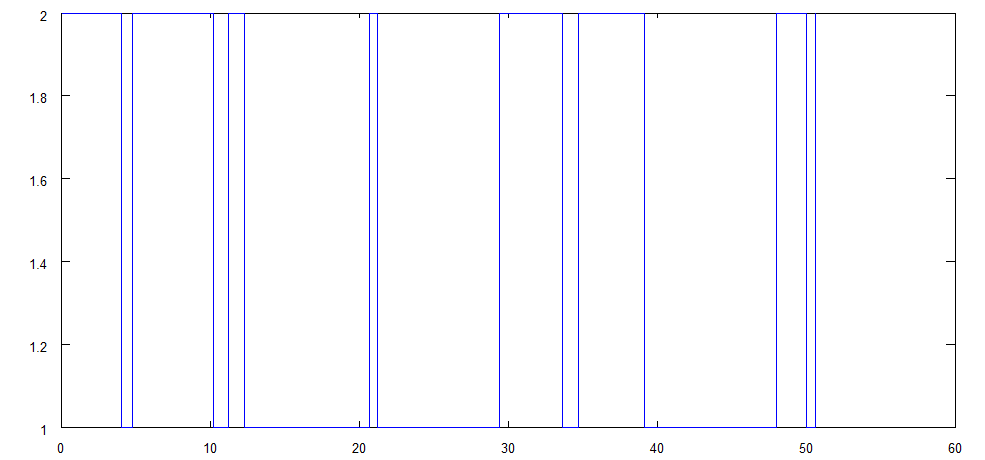
\includegraphics[width=0.7\textwidth]{7markov.png}
\caption{Simulaci\'on Markov}
\label{MarkovSim}
\end{figure}
\end{proof}
\item Utilice su programa para generar 10000 trayectorias en el intervalo de tiempo $[0,10]$ comenzando con probabilidad $1/2$ en cada estado y obtenga la distribuci\'on emp\'irica de $X_10$. 
\begin{proof}
El c\'odigo utilizado ser\'a el siguiente,
\begin{lstlisting}
l(1)=2;
l(2)=3;
t=10;
edos=zeros(1,2);
for j=1:1000
T=[];
N=[];
s=0;
edo=1;
ifunifrnd(0,1)<0.5
edo=edo+1;
endif
i=1;
N(i)=edo;
T(i)=exprnd(l(edo));
while s<t
N(i+1)=abs(N(i)-2) +1;
T(i+1)=T(i) + exprnd(l(N(i+1)));
s=T(i+1);
i=i+1;
endwhile
edos(N(i-1))=edos(N(i-1))+1;
endfor
\end{lstlisting}
El n\'umero total de veces que al tiempo $t$ est\'a en el estado $k$ es la variable $edos(k)$ para $k=1,2$. En la trayectoria realizada, se obtuvo que $edos(1)=5933$ y $edos(2)=4067$.
\end{proof}
\item Calcule $e^{10Q}$ (utilizando alg\'un comando adecuado) y contraste con la distribuci\'on emp\'irica del inciso anterior.
\begin{proof}
\begin{lstlisting}
Q=[-2,2;3,-3];
pi=[0.5, 0.5];
t=10;
Q=Q*t;
Q=expm(Q);
prob=pi*Q;
\end{lstlisting},
dando como resultado que
\[e^{tQ}=\begin{pmatrix}
0.6 & 0.4 \\ 
0.6 & 0.4
\end{pmatrix}.\]
\end{proof}
\item Codifique el siguiente esquema num\'erico, conocido como m\'etodo de Euler, para aproximar a $e^{10 Q}$: escoja $h>0$ peque\~no, defina a $P^h_0$ como la matriz identidad y recursivamente\begin{esn}
P^h_{i+1}=P^h_i+hQP^h_i. 
\end{esn}corra hasta que $i=\floor{10/h}$ y compare la matriz resultante con $e^{10Q}$. Si no se parecen escoja a $h$ m\'as peque\~no. ?`Con qu\'e $h$ puede aproximar a $e^{10Q}$ a 6 decimales?
\end{enumerate}
\begin{proof}
El c\'odigo ser\'a
\begin{lstlisting}
Q=[-2,2;3,-3];
P=eye(2);
h=0.33;
i=1;
while i<= floor(10/h)
P=P+h*Q*P;
i=i+1;
endwhile
\end{lstlisting}
Este algoritmo se acerca al valor real cuando $h=0.3$ (de hecho, Octave se�ala que es el mismo). Sin embargo, se probaron valores como $0.4$ que daba valores que ni siquiera correspond\'ian a una probabilidad. El valor que se detecto era bueno sin un cambio tan brusco era justamente 0.33.
\end{proof}
\end{problema}

\bibliography{GenBib}
\bibliographystyle{amsalpha}
\end{document}
